\documentclass[10pt]{article}
\usepackage[T1]{fontenc}
\usepackage[utf8]{inputenc}
\usepackage[margin=0.8in]{geometry}
\usepackage{amsmath,amssymb}
\usepackage{booktabs}
\usepackage{longtable}
\usepackage{array}
\usepackage{graphicx}
\usepackage{float}
\usepackage{placeins}
\usepackage{xcolor}
\usepackage{enumitem}
\usepackage{hyperref}
\graphicspath{{figures/}}
\setlist{itemsep=1pt,topsep=2pt}
\emergencystretch=3em

% ------------------------------------------------------------------ notation
\newcommand{\code}[1]{\texttt{#1}}
\newcommand{\feat}[2]{\par\medskip\noindent\textbf{\texttt{#1}}\hfill{\small [#2]}\par\nopagebreak\smallskip}
\newcommand{\med}{\operatorname*{median}}
\newcommand{\mean}{\operatorname*{mean}}
\newcommand{\std}{\operatorname{sd}}
\newcommand{\rsd}{\operatorname{rsd}}
\newcommand{\argmax}{\operatorname*{arg\,max}}
\newcommand{\argmin}{\operatorname*{arg\,min}}
\newcommand{\Dt}{\mathcal D}
\newcommand{\nw}{n_\text{w}}
\newcommand{\kt}{k_\text{t}}
\newcommand{\ko}{k_0}
\newcommand{\G}{\mathcal G}

\title{Trace Features: Technical Definitions\\[2pt]
\large How every feature of \code{trace\_features.py} is computed}
\author{ML-assisted optimization of CCD operating parameters --- technical note\\
\small companion to ``Trace Features for Machine Learning: the Complete List''}
\date{14 October 2026; updated 22 October 2026}

\begin{document}
\maketitle

\begin{abstract}
The first note on the trace features (\code{docs/overleaf\_trace\_features/trace\_features.tex}) lists the scalar features and curves with a one-line
description each. This note gives the mathematics: since 22 October 2026 for all 141 scalars and 18 curves, the original 85 and 14 and
the 56 scalars and 4 curves added on 2026-10-21/22 (Section~\ref{sec:extra}). It covers:
\begin{itemize}
\item how a raw trace is turned into skip cycles, CDS values and transfers;
\item the common operations (robust statistics, detrending, spectra, Allan deviation, step statistics, the fitting procedures);
\item the exact formula of every feature and curve, with the index ranges and constants used in the code;
\item the implementation tiers and how the evidence tiers that choose each model's features are computed (Section~\ref{sec:tiers}).
\end{itemize}
All counts are given for a general trace. The values for the usual trace geometry (2$\times$5 pixels, 500 skips,
150-sample windows) are in brackets. The equations follow \code{src/trace\_regions.py}, \code{src/compare\_trace.py} and
\code{src/trace\_features.py} and \code{src/trace\_features\_extra.py} (version of 2026-10-22); where the code makes a choice (a degree of freedom, a tolerance), it is
stated.
\end{abstract}

\tableofcontents

%======================================================================
\section{The trace and its notation}

\subsection{Samples, windows and cycles}
A trace is the ADC output of one channel at $f_s = 15$\,MHz: samples $v_t$ in ADU, $t = 0, 1, \dots$, with
$\Delta t = 1/f_s = 66.7$\,ns. Each sample carries flag bits from the sequencer. Bit 0 (RD) is high in the pedestal window, bit 1
(RU) in the signal window, bit 6 during the first part of each horizontal transfer, and bit 7 during the first part of each
vertical transfer. After every window, the ADC writes an inline record with the window's sample sum $\Sigma$ and length $n$.

\paragraph{Pixels and skips.} The pedestal and signal windows are taken in time order. A pixel is $N$ (pedestal, signal) pairs
followed by one extra pedestal window, so a pixel ends where a pedestal window is followed by another pedestal window. This gives pixels
$p = 0, \dots, N_p - 1$ [10] and skips $k = 0, \dots, N - 1$ [500] (\code{NDCM}). Let $t^\text{ped}_{p,k}$ be the first sample of
the pedestal window of skip $k$.

\paragraph{Cycle length.} With $\delta = t^\text{ped}_{p,k+1} - t^\text{ped}_{p,k}$ over all pixels and skips,
\begin{equation}
P = \med \delta \quad[488], \qquad P_\text{exact} = \mean\{\delta : |\delta - P| \le 1\} \quad[488.7].
\end{equation}
The cycle is not a whole number of samples (3258 sequencer ticks of 10\,ns $= 488.7$ samples), so the window starts walk by a third of a
sample from skip to skip. The window length is $\nw = \med(\text{pedestal end} - \text{start})$ [150]; the signal-window offset is
$s = \med(t^\text{sig}_{p,k} - t^\text{ped}_{p,k})$ [207]; the signal window ends at $e = \min(s + \nw, P)$ [357].

\paragraph{Cycle matrix, baseline, shape.} For pixel $p$ (index $p$ dropped when clear):
\begin{align}
Y_{k,\tau} &= v_{t^\text{ped}_{p,k} + \tau}, \qquad \tau = 0, \dots, P-1 \qquad\text{(one row per skip)},\\
b_k &= \frac{1}{\nw}\sum_{\tau=0}^{\nw-1} Y_{k,\tau} \qquad\text{(the skip's baseline: its pedestal-window mean)},\\
X_{k,\tau} &= Y_{k,\tau} - b_k \qquad\text{(shape with the baseline removed)}.
\end{align}

\paragraph{CDS.} From the inline records, the correlated double sample of skip $k$ is
\begin{equation}
c_k = \frac{\Sigma^\text{ped}_k}{n^\text{ped}_k} - \frac{\Sigma^\text{sig}_k}{n^\text{sig}_k}\qquad\text{(ADU)},
\end{equation}
pedestal minus signal, so that charge (which lowers the signal level) gives a positive CDS.

\paragraph{Transfers.} In the gap before each pixel, the rising edges of bit 6 mark horizontal transfers. They are stacked into
$H^{(p)}_{m,\tau}$, $m = 1\dots M_p$ (transfer) [19 complete ones], $\tau = 0\dots L_H - 1$. The rising edges of bit 7 mark vertical
transfers (bit 5 if bit 7 has fewer than two edges; an edge counts only if the bit stays high for $\ge 10$ samples), stacked into
$V_{m,\tau}$, $\tau < \mathrm{round}(P_V)$ ($P_V$: median spacing of the vertical edges), for the vertical block before the first row-start
pixel after pixel 0 (else the leading block), using only transfers that end before that gap's first horizontal edge. The first transfer
of the block is dropped when there are at least three, because it follows the skip region. The trace usually \emph{starts} inside a vertical
block (the leading block, before pixel 0), at a random point: only part of its transfers are recorded.

\subsection{Pixel sets and counts}
\paragraph{Row-start pixels} $\mathcal S$ are pixel 0 and every pixel read right after vertical transfers ($p \bmod \code{NCOL} = 0$ from
the \code{.meta}).

\paragraph{Usable pixels} $\G$ are the other pixels, minus pixels holding a large charge. With
$\bar c_p = \mean_{k \ge \ko} c_{p,k}$ over the non-row-start candidates,
\begin{equation}
p \in \G \iff |\bar c_p - \med_q \bar c_q| < 8 \max\bigl(1.4826\,\med_q |\bar c_q - \med_{q'} \bar c_{q'}|,\; 5\ \text{ADU}\bigr).
\end{equation}
If every pixel starts a row (one column), all pixels are candidates.

\paragraph{Counts} (\code{trace\_sizes}, \code{skip\_counts}), all derived from the trace:
\begin{center}
\small
\begin{tabular}{llll}
\toprule
Symbol & Meaning & Definition & [usual] \\
\midrule
$\kt$ & first skip in mean shapes & $\min(5, \lfloor N/10\rfloor)$ & [5] \\
$\ko$ & first skip in noise features & $\min(10, \lfloor N/10\rfloor)$ & [10] \\
$n_r$ & skips in the ringing fit & $\min(20, \lfloor N/2\rfloor)$ & [20] \\
$K$ & a tenth of the skips & $\max(1, \lfloor N/10\rfloor)$ & [50] \\
$B$ & noise block & $50$ if $N - \ko \ge 250$, else $\max(2, \lfloor (N-\ko)/5\rfloor)$ & [50] \\
$w$ & step window & $\min(20, \lfloor (N-\ko)/10\rfloor)$ & [20] \\
$k_\text{ets}$ & first skip for equivalent time & $\lfloor N/5\rfloor$ & [100] \\
$q$ & settling samples & $\min(10, \max(1, \lfloor\nw/10\rfloor))$ & [10] \\
$L_h$ & half window & $\max(1, \lfloor \nw/2\rfloor)$ & [75] \\
$\mathcal L$ & window lengths & $\{\max(1, \mathrm{round}(f\,\nw)) : f \in \{10,20,30,50,75,100,125,150\}/150\}$ & [10\dots150] \\
\bottomrule
\end{tabular}
\end{center}
A feature that needs more skips, pixels or transfers than the trace has is NaN.

%======================================================================
\section{Common operations}

\paragraph{Aggregation over pixels.} A \emph{per-pixel} feature $f_p$ is computed for each $p \in \G$, and the trace's value is
\begin{equation}
F = \med_{p \in \G} f_p, \qquad \text{spread} = \rsd_{p\in\G}(f_p),\quad \rsd(x) = 1.4826\,\med_i |x_i - \med_j x_j|.
\end{equation}
The factor $1.4826 = 1/\Phi^{-1}(0.75)$ makes $\rsd$ equal to the standard deviation for Gaussian data: $P(|X - \mu| < 0.6745\sigma) = 0.5$.
Unlike the standard deviation, a few outlying pixels barely change it.

\paragraph{Polynomial detrending.} For a sequence $x_0 \dots x_{n-1}$,
\begin{equation}
\Dt(x)_k = x_k - \sum_{j=0}^{d} \hat\beta_j u_k^j,\qquad u_k = \frac{k - n/2}{n/2},\qquad d = \min\bigl(4, \lfloor n/50\rfloor\bigr),
\end{equation}
where $\hat\beta$ is the least-squares fit. A degree-4 polynomial removes variations slower than about a quarter of the record (drift,
droop) but keeps the noise of averages over up to $\sim$50 skips. A running mean is \emph{not} used: subtracting a running mean of
length $n$ would cancel the averages over $n$ skips and make their noise look far too small.

The detrended CDS of pixel $p$ is $r_{p,k} = \Dt(c_{p,\ko:})_k$, $k = 0 \dots N - \ko - 1$ [490 values].

\paragraph{Residual cycles.} At each position $\tau$ of the cycle, a polynomial of degree $d$ in the (standardized) skip index is
fitted across the skips $k \ge \ko$ and removed:
\begin{equation}
R_{k,\tau} = Y_{\ko+k,\tau} - \sum_{j=0}^{d} \hat\gamma_{j\tau}\, u_k^j .
\end{equation}
This removes the mean waveform and its slow change along the pixel (the droop), and leaves the skip-to-skip variation.

\paragraph{Block noise.} The noise of an $n$-skip average is the standard deviation of the means of consecutive blocks,
\begin{equation}
\sigma(n) = \std_{j}\Bigl(\tfrac{1}{n}\textstyle\sum_{i=0}^{n-1} r_{jn+i}\Bigr) \quad(\text{ddof} = 1),
\end{equation}
undefined with fewer than 3 blocks. For white noise $\sigma(n) = \sigma(1)/\sqrt n$.

\paragraph{Autocorrelation} at lag $\ell$ of a sequence $x$ (mean removed, $\tilde x = x - \bar x$):
$\rho(\ell) = \sum_{k} \tilde x_k \tilde x_{k+\ell} \big/ \sum_k \tilde x_k^2$.

\paragraph{Allan deviation.} With $\bar x^{(n)}_j$ the means of consecutive $n$-blocks ($m = \lfloor N'/n\rfloor$ blocks; needs $m > 2$),
\begin{equation}
\sigma_A(n) = \sqrt{\tfrac12\,\mean_j\bigl(\bar x^{(n)}_{j+1} - \bar x^{(n)}_j\bigr)^2},\qquad n \in \{1,2,3,5,7,10,15,20,30,50,75,100,160\}.
\end{equation}
White noise gives $\sigma_A \propto n^{-1/2}$; anticorrelated noise falls faster; $1/f$ noise flattens.
Applied to the detrended $r_p$, points with $n > N'/5$ are biased low: the degree-4 polynomial absorbs most of the difference between
3 or 4 block means (at $n = 160$, $N' = 490$: about 0.4 of the white-noise value on the 2026-10-12 traces). Fits use $n \le N'/5$.

\paragraph{Overlapping Allan deviation.} With the running means $\tilde x^{(n)}_i = \tfrac1n\sum_{l=0}^{n-1} x_{i+l}$ over \emph{every} start
$i = 0 \dots N'-n$,
\begin{equation}
\sigma^\text{ov}_A(n) = \sqrt{\tfrac12\,\mean_{i=0}^{N'-2n}\bigl(\tilde x^{(n)}_{i+n} - \tilde x^{(n)}_i\bigr)^2}
\end{equation}
(same $n$, undefined when $\lfloor N'/n\rfloor \le 2$): the same expectation as $\sigma_A$, with much less scatter for long blocks.

\paragraph{CDS with the common pattern removed.} With $\G$ the usable pixels ($P = |\G|$) and $\bar c_k = \mean_{q \in \G} c_{q,k}$,
\begin{equation}
u_{p,k} = \sqrt{\tfrac{P}{P-1}}\;\Bigl[(c_{p,k} - \bar c_k) - \mean_{k' \ge \ko}(c_{p,k'} - \bar c_{k'})\Bigr],\qquad k \ge \ko .
\end{equation}
The pattern along the skips that every pixel shares (droop, charge collection) is not noise for an image: it shifts every pixel alike.
No polynomial is removed, so slow noise that differs from pixel to pixel (a floor that does not average down) stays in $u_p$, as it
does in an image. The factor $\sqrt{P/(P-1)}$ restores the white-noise level ($c_{p} - \bar c$ has variance $(1 - 1/P)\sigma^2$).

\paragraph{Spectral density} of $M$ equal-length sequences $x^{(m)}$ of length $n$, sampled at rate $f_r$, with a Hann window $h$:
\begin{equation}
S(f_j) = \frac{2}{f_r\sum_k h_k^2}\;\mean_m \Bigl|\sum_k h_k x^{(m)}_k e^{-2\pi \mathrm{i}\, jk/n}\Bigr|^2,\qquad f_j = j f_r/n,
\end{equation}
a one-sided density in ADU$^2$/Hz. For the CDS the rate is the skip rate $f_\text{skip} = f_s/P_\text{exact}$ [30.69\,kHz].

\paragraph{Largest step.} For a sequence $x$ and window $w \ge 3$, at every $k \in [w, n - w)$ the means and variances of the $w$ values
before and after are compared:
\begin{equation}
t_k = \frac{|\bar x_{[k,k+w)} - \bar x_{[k-w,k)}|}{\sqrt{(s^2_{[k-w,k)} + s^2_{[k,k+w)})/w}},\qquad T = \max_k t_k .
\end{equation}
For Gaussian white noise the maximum over $\sim$470 positions is about 4; a telegraph (two-level) process gives much larger values.

\paragraph{Spectral lines.} In a spectrum $S_i$, bin $i$ is a line if $S_i > 5\,\med\{S_{i-5..i-1}, S_{i+1..i+5}\}$ and $S_i$ is the
largest of $S_{i-1..i+1}$; the feature is the number of lines.

\subsection{Fitting procedures}
\paragraph{One exponential (variable projection).} To fit $y(x) = A e^{-x/\tau} + C$:
\begin{enumerate}
\item For each trial $\tau$ on a logarithmic grid of 60 values in $[\tau_\text{min}, \tau_\text{max}]$, $A$ and $C$ enter linearly and
  are solved exactly by least squares. The residual sum of squares is $Q(\tau) = \min_{A,C}\sum_i (y_i - Ae^{-x_i/\tau} - C)^2$.
\item The best grid value is refined on 41 log-spaced values in $[\tau/1.25, 1.25\tau]$.
\item A parabola through $Q$ at the best point and its two neighbours, in $\log\tau$, gives
  $\log\hat\tau = \log\tau_i + \tfrac12\Delta\,(Q_{i-1} - Q_{i+1})/(Q_{i-1} - 2Q_i + Q_{i+1})$, with $\Delta$ the grid step in $\log\tau$.
\end{enumerate}
Reported: $\hat\tau$, $\hat A$ (and $\hat C$). The parabola removes the quantization to the grid, which would otherwise make repeats
give identical values.

\paragraph{Two exponentials.} $y = A_1 e^{-x/\tau_1} + A_2 e^{-x/\tau_2} + C$ with $\tau_1 < \tau_2$:
\begin{itemize}
\item all pairs from a 40-value log grid in $[0.5, 200]$ samples;
\item a 21$\times$21 log grid between the neighbouring grid values of the best pair;
\item a parabola in $\log\tau$ for each time constant;
\item the refined pair is kept only if it does not increase $Q$.
\end{itemize}

\paragraph{Damped ringing} (corrected 2026-10-13). For $y_k = c_k - \med_{k' \ge \ko} c_{k'}$, $k = 1 \dots n_r - 1$:
\begin{equation}
y_k = C + e^{-k/\tau}\bigl(a\cos 2\pi f k + b\sin 2\pi f k\bigr).
\end{equation}
$C, a, b$ are linear and solved for every $(f, \tau)$ pair, using normal equations for all pairs at once. The grid is $f \in [0.02, 0.5]$
cycles/skip (97 values) and $\tau \in [0.5, 30]$ skips (31 log values). It is refined on $25\times25$ points within
$f \pm 0.006$, $\tau \times 1.2^{\pm1}$, then by a parabola in $f$. Skip 0 is left out (it has its own feature). $C$ absorbs the level that
has not yet settled. Reported: $f$, $\tau$, $\sqrt{a^2+b^2}$. Below $f = 0.02$ (a period longer than 50 skips) an oscillation cannot be
told from $C$ in 20 skips.

\paragraph{Noise model.} $\sigma(n)^2 = \sigma_w^2/n + \sigma_f^2$ is linear in $(\sigma_w^2, \sigma_f^2)$. It is fitted by least squares
to the block noise at $n \in \{1, 2, 5, 10, 25, 50\}$ (those with $\ge 3$ blocks), and the coefficients are clipped at 0.

\paragraph{Interpolated crossings and peaks.} A level crossing between samples $i-1$ and $i$ is placed at
$x_{i-1} + (\ell - y_{i-1})(x_i - x_{i-1})/(y_i - y_{i-1})$. A spectral peak at bin $i$ is refined with the parabola through the
log-powers $a, b, c$ of bins $i-1, i, i+1$: $f = f_i + \tfrac12 (a - c)/(a - 2b + c)\,\Delta f$.

%======================================================================
\section{Comparison tools: parametric fits (group \code{fit}, per pixel)}

The mean shape (template) of a pixel is $m_\tau = \mean_{k \ge \kt} X_{k,\tau}$. Times are converted with $1\,\mu\text{s} = 15$ samples.

\feat{fit: settling time after pulse (us)}{µs}
$i^\star = e + \argmax_{\tau \ge e} m_\tau$ (the reset-pulse maximum). Fit $m_\tau = A e^{-x/\tau_s} + C$ for $\tau \ge i^\star$,
$x = (\tau - i^\star)/15$\,µs, with $\tau_s \in [0.05, 20]$\,µs. The feature is $\tau_s$; \code{fit: settling amplitude after pulse} is $A$ (ADU).

\feat{fit: dip recovery time (us)}{µs}
$i_d = \nw + \argmin_{\nw \le \tau < s} m_\tau$ (the bottom of the summing-well dip). Fit $m_\tau$ for $i_d \le \tau < s$ with
$\tau_d \in [0.02, 10]$\,µs. Feature $\tau_d$; \code{fit: dip recovery amplitude} is $A$. Undefined if $s \le \nw + 5$.

\feat{fit: baseline droop time constant (skips)}{skips}
Fit $b_k = A e^{-k/\tau_b} + C$ for $k = 1 \dots N-1$, $\tau_b \in [\min(5, \max(1, \lfloor N/100\rfloor)),\ \max(5000, 10N)]$.
Feature $\tau_b$; \code{fit: baseline droop amplitude} is $A$ (negative when the baseline rises).

\feat{fit: first-skip ringing frequency (cyc/skip)}{cycles/skip}
The damped-ringing fit of Section~2 on the first $n_r$ CDS values: $f$. \code{decay (skips)} is $\tau$; \code{amplitude} is $\sqrt{a^2+b^2}$
(the envelope extrapolated to skip 0).

\feat{fit: white noise per skip (ADU)}{ADU}
$\sigma_w$ of the noise model; \code{fit: correlated noise floor (ADU)} is $\sigma_f$, the part that averaging over skips does not remove.

%======================================================================
\section{Comparison tools: skip-cycle tools (group \code{skip}, per pixel)}

With $\mu = \min(10, \lfloor\nw/8\rfloor)$ and $\tilde c = \med_{k \ge \ko} c_k$:
\begin{center}
\small
\renewcommand{\arraystretch}{1.25}
\begin{longtable}{>{\raggedright\arraybackslash}p{0.33\textwidth}>{\raggedright\arraybackslash}p{0.6\textwidth}}
\toprule
Feature & Definition \\
\midrule
\endhead
\code{skip: dip height} & $\min_{\nw \le \tau < s} m_\tau$ \\
\code{skip: signal-window level} & $\mean_{s+\mu \le \tau < e - \mu} m_\tau$ (the signal level relative to the pedestal, inside the window) \\
\code{skip: pulse peak height} & $\max_{\tau \ge e} m_\tau$ \\
\code{skip: end-of-cycle tail level} & mean of the last $\min(30, \max(1, \lfloor(P - e)/4\rfloor))$ values of $m_\tau$ \\
\code{skip: baseline at skip 1} & $b_1$ \\
\code{skip: droop total} & $\Delta_b = b_{N-1} - b_1$ \\
\code{skip: droop half-time (skips)} & $\min\{j \ge 0 : (b_{1+j} - b_1)\,\mathrm{sgn}\,\Delta_b \ge |\Delta_b|/2\}$ \\
\code{skip: CDS mean (skips>=10)} & $\mean_{k \ge \ko} c_k$ \\
\code{skip: CDS rms (detrended)} & $\std(r)$, ddof $=1$ \\
\code{skip: first-skip CDS excess} & $c_0 - \tilde c$ \\
\code{skip: skips 1-4 CDS ringing} & $\sqrt{\tfrac14 \sum_{k=1}^{4}(c_k - \tilde c)^2}$ \\
\code{skip: CDS autocorrelation at lag 2} & $\rho(2)$ of $r$ \\
\code{skip: noise of 10-skip average} & $\sigma(10)$ of $r$ \\
\code{skip: noise of 50-skip average} & $\sigma(50)$ of $r$ \\
\code{skip: noise power 0.1-1 MHz} & $\log_{10}\sum_{f_j \in [0.1, 1)\,\text{MHz}} \Pi(f_j)$, see below \\
\code{skip: noise power 1-3 MHz} & same, $[1, 3)$\,MHz \\
\code{skip: noise power 3-7.5 MHz} & same, $[3, 7.51)$\,MHz \\
\bottomrule
\end{longtable}
\end{center}
\textbf{Window noise power.} Inside the pedestal window, the noise left after removing the template is
$\omega_{k,\tau} = X_{k,\tau} - m_\tau$ ($k \ge \kt$, $\tau < \nw$), with each row's own mean removed, and
$\Pi(f_j) = \tfrac{1}{\nw}\mean_k |\sum_\tau \omega_{k,\tau} e^{-2\pi i j\tau/\nw}|^2$, $f_j = j f_s/\nw$ (100\,kHz bins for
$\nw = 150$).

%======================================================================
\section{Comparison tools: transfers (groups \code{horizontal}, \code{vertical})}

For a stack of transfers $T_{m,\tau}$ of length $L$, with $n_b = \min(30, \max(1, \lfloor L/10\rfloor))$ and
$n_e = \min(50, \max(1, \lfloor L/10\rfloor))$:
\begin{align}
h_{m,\tau} &= T_{m,\tau} - \tfrac{1}{n_b}\textstyle\sum_{\tau' < n_b} T_{m,\tau'}, \qquad \bar h_\tau = \mean_m h_{m,\tau},\\
\text{minimum} &= \min_\tau \bar h_\tau,\quad \text{maximum} = \max_\tau \bar h_\tau,\quad
\text{end level} = \tfrac{1}{n_e}\textstyle\sum_{\tau \ge L - n_e} \bar h_\tau,\\
\text{scatter between transfers} &= \med_\tau \std_m(h_{m,\tau}) \quad(\text{ddof}=1).
\end{align}
\textbf{Horizontal:} $T = H^{(p)}$, all transfers of one usable pixel; the trace value is the median over pixels.
\textbf{Vertical:} each transfer of the block is one replicate ($M = 1$), so there is no scatter; the trace value is the median over the transfers.

%======================================================================
\section{CDS level (group \code{level})}

\begin{figure}[H]
\centering
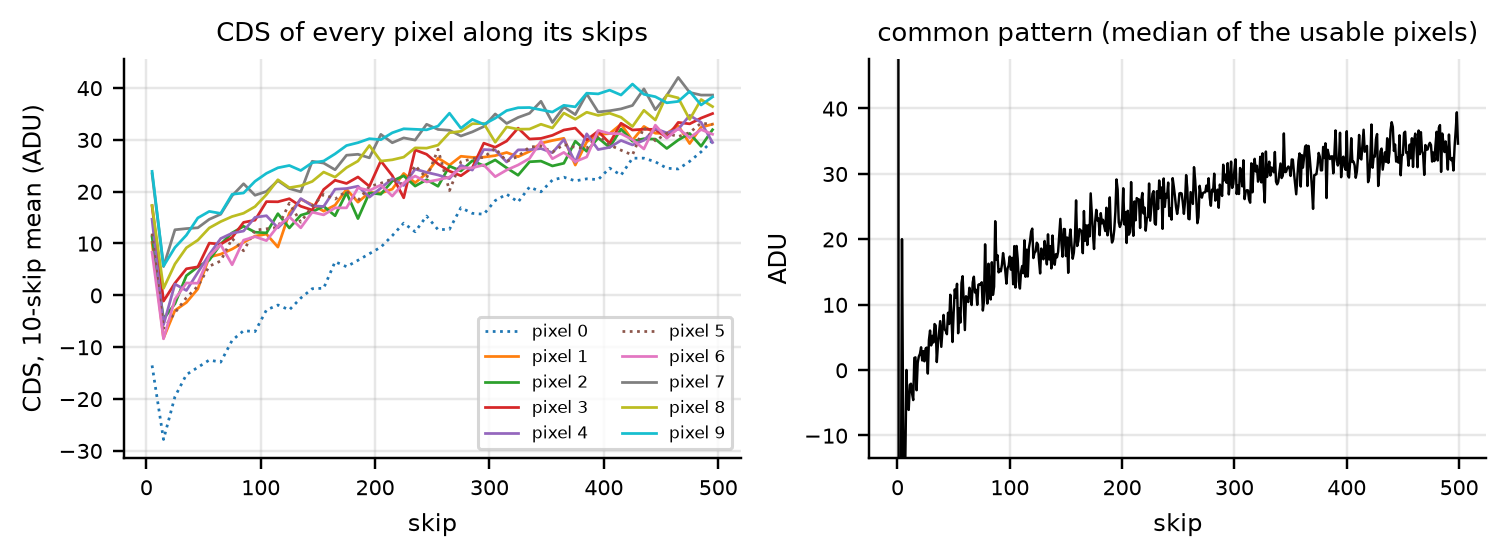
\includegraphics[width=\textwidth]{level_common_pattern.png}
\caption{Left: CDS of every pixel along its skips (10-skip means; dotted: row-start pixels). Right: the common pattern $\hat c_k$.
Example trace: module 101, channel 0, 2026-10-08, first repeat (all figures).}
\end{figure}

Common pattern and relative level:
\begin{equation}
\hat c_k = \med_{p \in \G} c_{p,k},\qquad \rho_p = \mean_{k \ge \ko}\bigl(c_{p,k} - \hat c_k\bigr).
\end{equation}
\feat{level: common CDS rise (ADU)}{ADU}
$\mean_{k \ge N - K} \hat c_k - \mean_{\ko \le k < \ko + K} \hat c_k$ [skips 450--499 minus 10--59].
\feat{level: pixel level spread (ADU)}{ADU}
$\rsd_{p \in \G}\, \rho_p$. With binning, each trace pixel holds the dark charge of $\code{NPBIN}\times\code{NSBIN}$ CCD pixels, so
this spread grows with the dark current.
\feat{level: pixel level max (ADU)}{ADU}
$\max_{p \in \G} \rho_p$.
\feat{level: charge-loss slope (\%)}{\%}
For every pixel (row starts included) with $\rho_p > 1000$\,ADU (charged): $d_k = c_{p,k} - \hat c_k$, $k \ge \ko$, $n' = N - \ko$;
straight-line fit $d_k \approx \alpha + \beta k$; loss $= 100\,\beta n'/\bar d$ (percent of the charge lost over the pixel). Median over
charged pixels; NaN if none.
\feat{level: charged-pixel skewness}{---}
$\mean(d - \bar d)^3/\std(d)^3$ for the same pixels; median.

%======================================================================
\section{Noise character (group \code{noise})}

\begin{figure}[H]
\centering
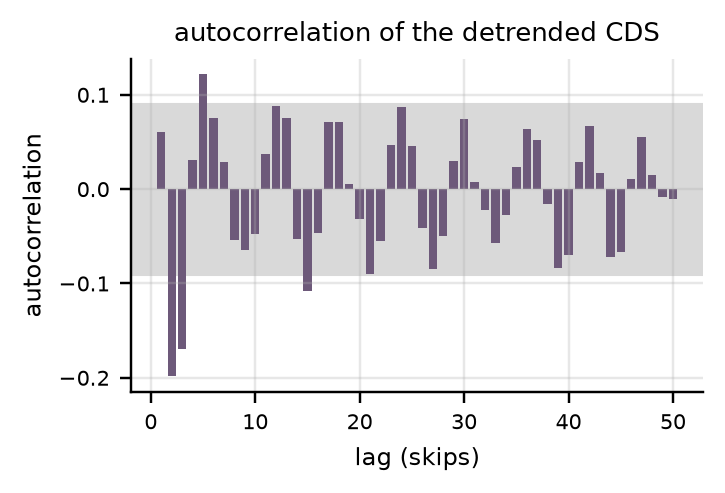
\includegraphics[width=0.5\textwidth]{noise_autocorrelation.png}\hfill
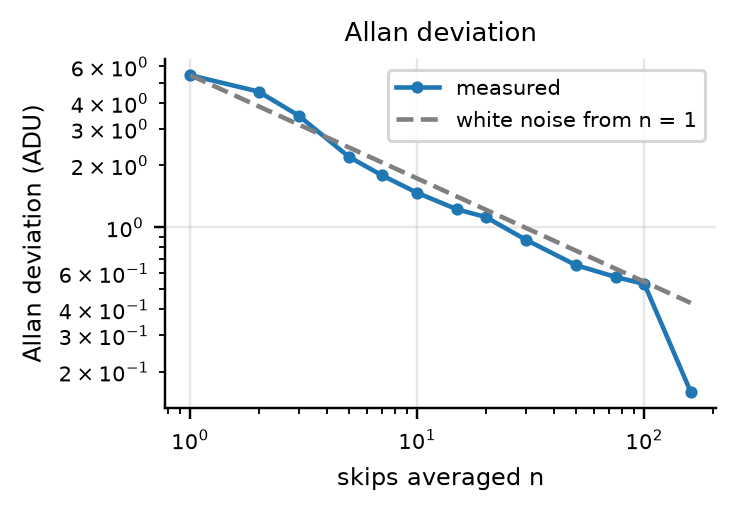
\includegraphics[width=0.48\textwidth]{noise_allan.png}
\caption{Left: autocorrelation of $r$ (mean of the usable pixels; grey band $\pm2/\sqrt{n}$). Right: Allan deviation with the white-noise line.}
\end{figure}

\feat{noise: CDS autocorrelation at lag 1}{---}
$\rho(1)$ of $r_p$; median over $\G$.
\feat{noise: Allan deviation n=50 (ADU)}{ADU}
$\sigma_A(50)$ of $r_p$; median. \code{noise: Allan slope n=10-100} $= \log_{10}\bigl(\sigma_A(100)/\sigma_A(10)\bigr)$ per pixel, median
(white noise: $-0.5$).
\feat{noise: CDS power <1 kHz / >10 kHz}{---}
With $S(f)$ the spectral density of the $r_p$ ($p \in \G$, needs $\ge 8$ values) at $f_\text{skip}$, and Nyquist frequency
$f_N = f_\text{skip}/2$, the bands are scaled to the usual $f_N^\text{ref} = 15.35$\,kHz so that they exist for any skip rate:
\begin{equation}
\frac{\mean\{S(f) : 0 < f < f_N \cdot 1/15.35\}}{\mean\{S(f) : f > f_N \cdot 10/15.35\}}
\quad\text{[exactly $<1$\,kHz over $>10$\,kHz at the usual rate]}.
\end{equation}
Low-frequency ($1/f$) noise raises it; white noise gives about 1.
\feat{noise: reset-level scatter (ADU)}{ADU}
$\std_k\bigl(\tfrac{1}{\nw}\sum_{\tau<\nw} R_{k,\tau}\bigr)$: the scatter of the level that each reset leaves, after the mean waveform
and the droop are removed. Median over $\G$. The CDS cancels it, because both windows of a skip share it.
\feat{noise: within-cycle power 0.1-0.3 MHz}{fraction}
On the segment $0 \le \tau < e$ (pedestal-window start to signal-window end): $u_{k,\tau} = R_{k,\tau} - \mean_{\tau'<e} R_{k,\tau'}$,
\begin{equation}
S_\text{in}(f_j) = \mean_{p}\mean_k\Bigl|\sum_{\tau<e} h_\tau u_{k,\tau} e^{-2\pi i j\tau/e}\Bigr|^2,\quad f_j = j f_s/e,\qquad
\text{feature} = \frac{\sum_{f_j \in [0.1, 0.3)\,\text{MHz}} S_\text{in}}{\sum_{f_j \ge 0.1\,\text{MHz}} S_\text{in}} .
\end{equation}
The \code{0.3-1}, \code{1-3} and \code{3-7.5\,MHz} features use the bands $[0.3,1)$, $[1,3)$ and $[3, 7.6)$\,MHz.

\begin{figure}[H]
\centering
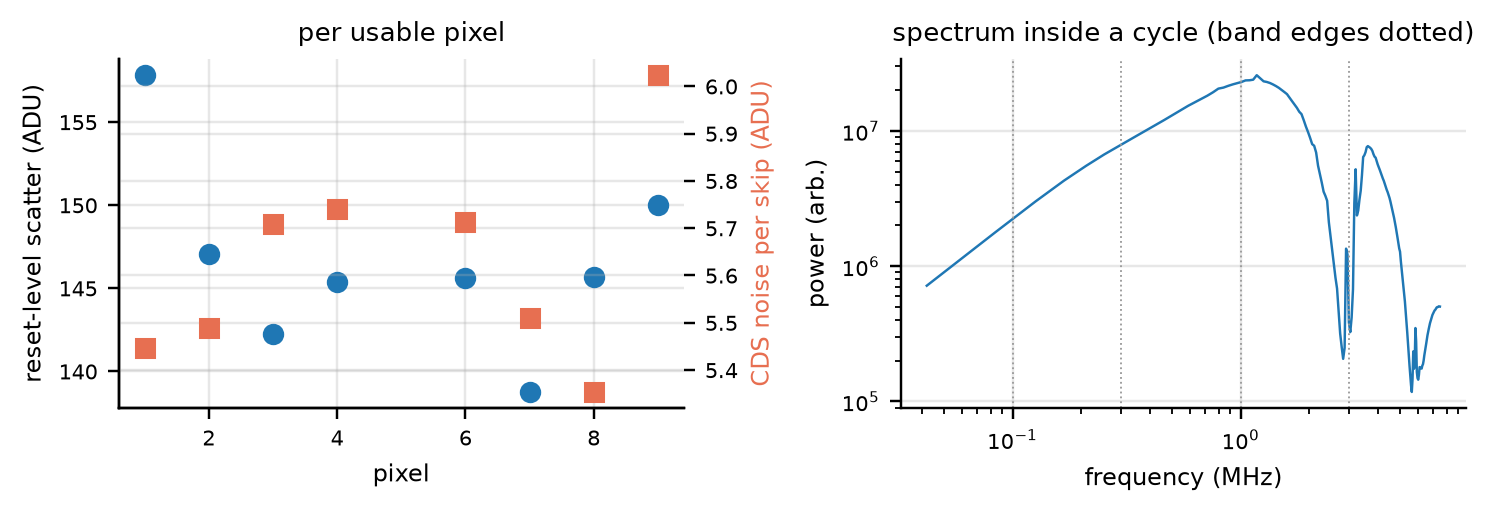
\includegraphics[width=\textwidth]{noise_reset_and_bands.png}
\caption{Left: reset-level scatter and CDS noise per skip for each usable pixel. Right: $S_\text{in}$ with the band edges.}
\end{figure}

\feat{noise: window-length ratio 75/150}{---}
The CDS recomputed from the raw samples with windows of $L$ samples starting $o$ samples into each window:
\begin{equation}
c^{(L,o)}_k = \tfrac{1}{L}\textstyle\sum_{\tau=o}^{o+L-1} Y_{k,\tau} - \tfrac{1}{L}\sum_{\tau=s+o}^{s+o+L-1} Y_{k,\tau},\qquad
\sigma(L,o) = \std\bigl(\Dt(c^{(L,o)}_{\ko:})\bigr)\ (\text{ddof }0).
\end{equation}
Feature $\sigma(L_h, 0)/\sigma(\nw, 0)$ per pixel, median (white noise: $\sqrt2$). \code{noise: late/early window ratio} is
$\sigma(L_h, \nw - L_h)/\sigma(L_h, 0)$: the second half of the windows against the first half (below 1 if the windows still settle at their
start). The curve \code{noise: noise vs window length} is $\mean_p \sigma(L, 0)$ for $L \in \mathcal L$.

\begin{figure}[H]
\centering
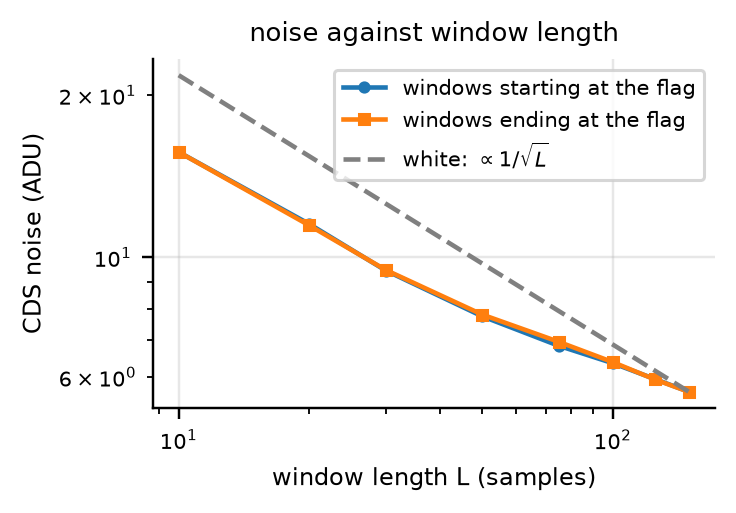
\includegraphics[width=0.5\textwidth]{noise_window_length.png}
\caption{$\sigma(L, 0)$ (circles) and $\sigma(L, \nw - L)$ (squares) against $1/\sqrt L$.}
\end{figure}

\feat{noise: pedestal-window settling (ADU)}{ADU}
The mean waveform inside the window, each skip's window mean removed:
$\bar W_\tau = \mean_{p}\mean_{k \ge \ko}\bigl(Y_{k,o+\tau} - \tfrac{1}{\nw}\sum_{\tau'}Y_{k,o+\tau'}\bigr)$, $\tau < \nw$, with $o = 0$.
Feature $\tfrac1q\sum_{\tau \ge \nw - q}\bar W_\tau - \tfrac1q\sum_{\tau<q}\bar W_\tau$. \code{signal-window settling} uses $o = s$.
\feat{noise: baseline coupling (1e-3)}{$\times10^{-3}$}
Slope $\gamma$ of $c_{p,k}$ against $b_{p,k}$ ($k \ge \ko$) by least squares, $\times10^3$; median. A slope means that the baseline (which
moves with each reset and droops) leaks into the CDS.
\feat{noise: noise trend along skips (ADU/100 skips)}{ADU/100 skips}
$s_j = \std(r_{jB:(j+1)B})$ for complete blocks; slope of $s_j$ against $jB$, $\times 100$ (needs $\ge 3$ blocks); median.

\begin{figure}[H]
\centering
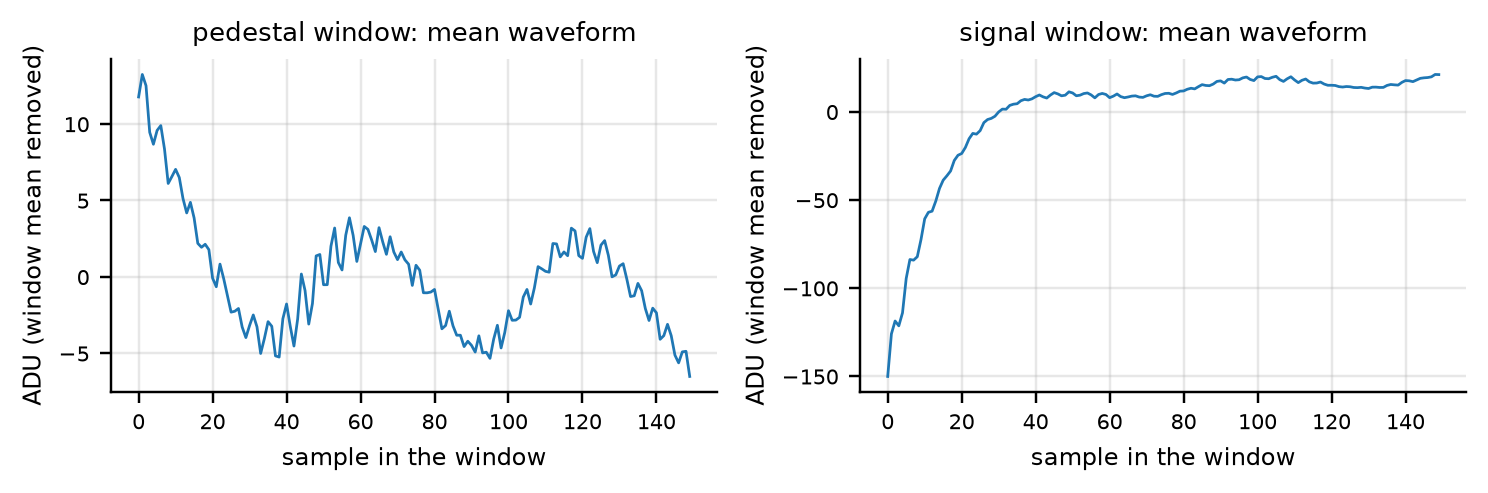
\includegraphics[width=\textwidth]{noise_window_settling.png}
\caption{$\bar W_\tau$ in the pedestal (left) and signal (right) windows.}
\end{figure}

%======================================================================
\section{Discrete and transient noise (group \code{discrete})}

\feat{discrete: largest baseline step (t)}{---}
$T$ (largest step, window $w$) of $\Dt(b_{\ko:})$; median over $\G$. \code{discrete: largest CDS step (t)}: $T$ of $r$.
\feat{discrete: CDS excess kurtosis}{---}
$\mean(\tilde r^4)/\mean(\tilde r^2)^2 - 3$ (0 for a Gaussian); median.
\feat{discrete: CDS outlier fraction}{fraction}
Fraction of $k$ with $|r_k - \med r| > 5\,\rsd(r)$; median.
\feat{discrete: CDS spectrum lines}{count}
Number of lines in $S(f)$ (excluding $f=0$). \code{discrete: within-cycle spectrum lines}: lines in $S_\text{in}$.
\feat{discrete: ADC low-bit chi2/dof}{---}
All pedestal-window samples of the usable pixels, $n_\text{tot}$ of them: counts $n_j$ of $v \bmod 64 = j$,
$\chi^2/\text{dof} = \tfrac{1}{63}\sum_{j=0}^{63}(n_j - n_\text{tot}/64)^2/(n_\text{tot}/64)$. A flat distribution of the low bits gives
about 1; missing or doubled ADC codes give more.

\begin{figure}[H]
\centering
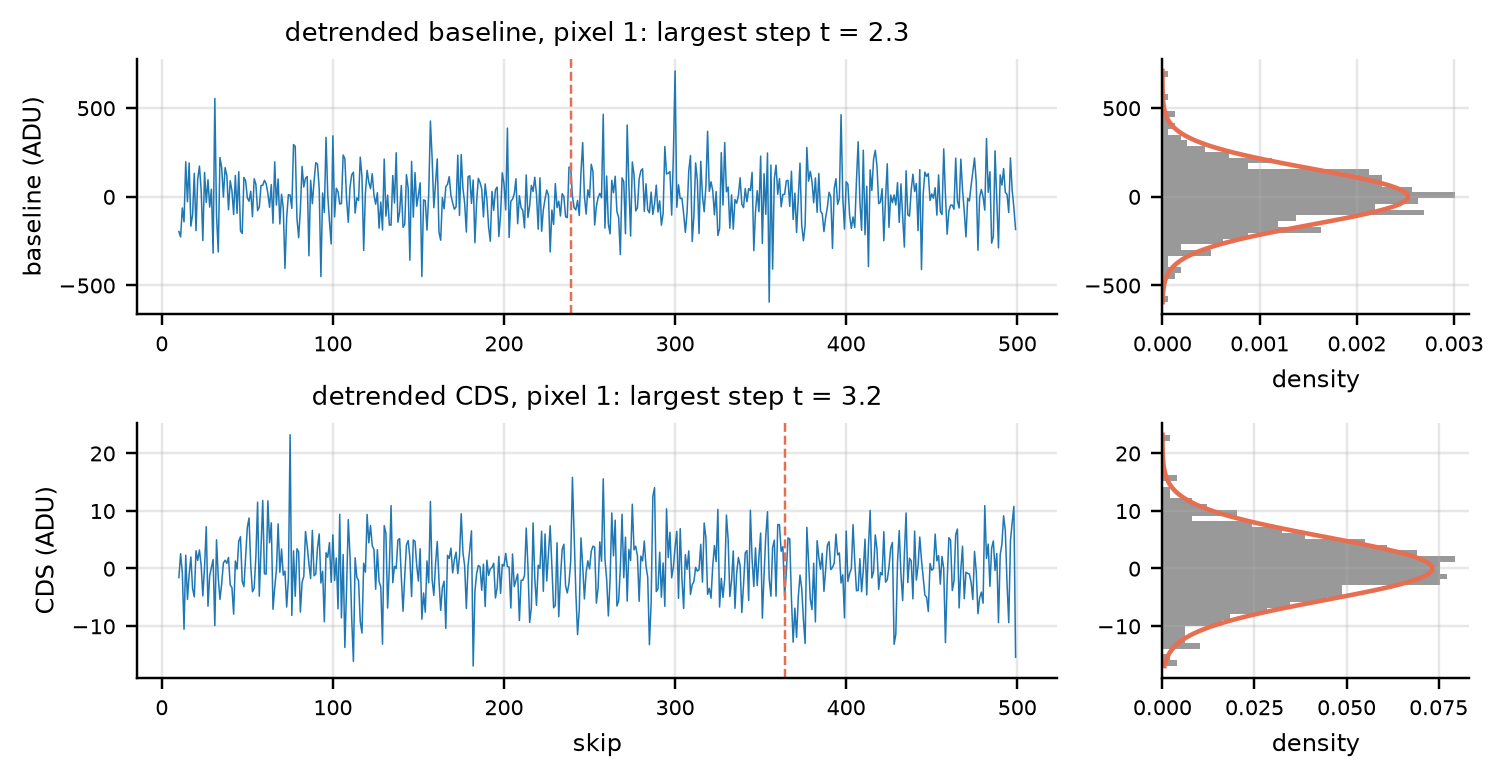
\includegraphics[width=\textwidth]{discrete_steps.png}
\caption{Detrended baseline and CDS of one pixel, with the largest step (dashed) and their distributions against a Gaussian.}
\end{figure}

%======================================================================
\section{Edges (group \code{edge})}
\label{sec:edges}

\paragraph{Pulse window.} With the mean shape over usable pixels $M_\tau = \mean_p m^{(p)}_\tau$, the pulse peak is
$\tau_\text{pk} = e + \argmax_{\tau \ge e} M_\tau$. The edge is searched in $[\ell_o, \ell_h)$ with
$\ell_o = \max(e - 7, \tau_\text{pk} - 30)$ and $\ell_h = \min(P, \tau_\text{pk} + 46)$. The level before the edge is the mean over
$[\max(s, \ell_o - 10), \ell_o + 6)$.

\paragraph{Edge times.} In each skip, with $y = Y_{k,\ell_o:\ell_h}$, the peak $i = \argmax y$ and the half-height
$\lambda = (\bar y_\text{before} + y_i)/2$, the last sample $j \le i$ below $\lambda$ gives
\begin{equation}
t^\text{edge}_k = t^\text{ped}_{p,k} + \ell_o + j + \frac{\lambda - y_j}{y_{j+1} - y_j}\qquad\text{(absolute sample time)}.
\end{equation}
A straight line $t^\text{edge}_k \approx \alpha k + \beta$ is fitted for $k \ge \min(5, \lfloor N/10\rfloor)$.

\feat{edge: jitter (ns)}{ns}
$\std_k\bigl(t^\text{edge}_k - \alpha k - \beta\bigr)\cdot 10^9/f_s$; median over pixels.
\feat{edge: period offset (1e-3 samples)}{$10^{-3}$ samples}
$10^3(\alpha - P_\text{expected})$, with $P_\text{expected}$ the cycle from the \code{.meta} sequencer formula (else $P_\text{exact}$).

\begin{figure}[H]
\centering
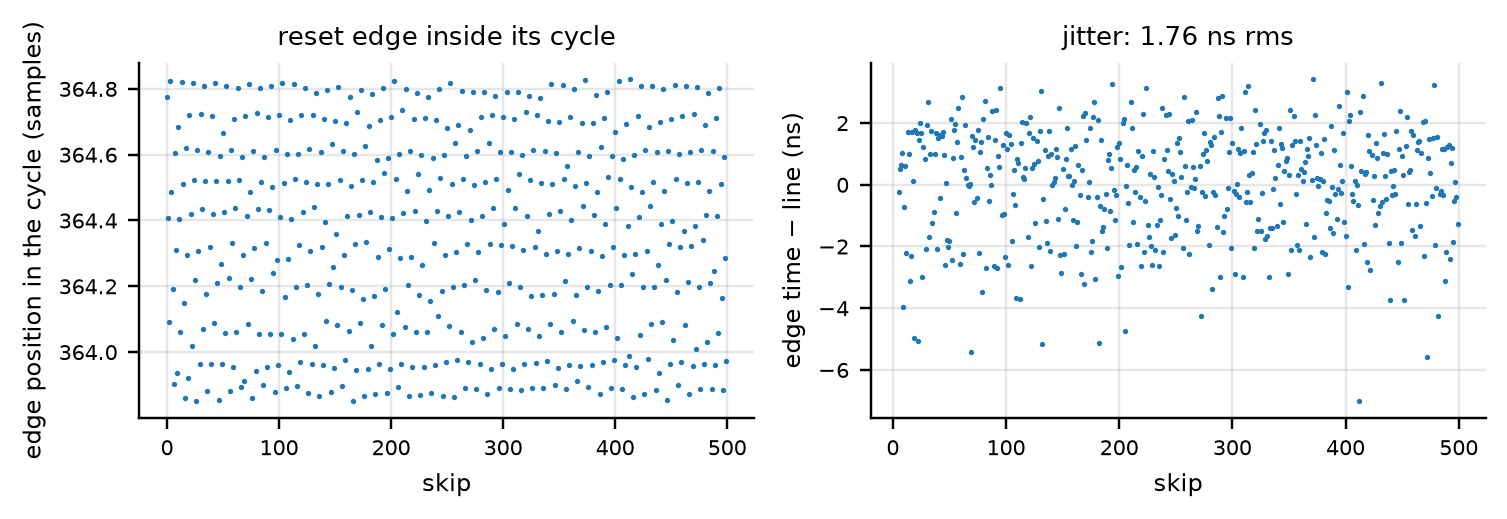
\includegraphics[width=\textwidth]{edge_jitter.png}
\caption{Left: the edge position inside its own cycle saws by a third of a sample, because the cycle is 488.7 samples long. Right:
residuals from the line.}
\end{figure}

\paragraph{Equivalent-time pulse.} Every sample of skips $k \ge k_\text{ets}$ of the usable pixels is placed at its time relative to
the fitted edge line, $\phi = t^\text{ped}_{p,k} + \tau - (\alpha k + \beta)$, and kept if $-15 < \phi < 60$. The values
$Y_{k,\tau} - b_k$ are averaged in 0.1-sample bins of $\phi$, giving $E(\phi)$: the pulse at 10$\times$ the sampling resolution. This
works because the 0.7-sample fractional part of the cycle spreads the samples over all phases.

\feat{edge: rise time (ns)}{ns}
$(\phi_{90} - \phi_{10})\cdot 10^9/f_s$, the interpolated crossings of 10\,\% and 90\,\% of $\max E$ on the rising side.
\feat{edge: recovery tau1 (us)}{µs}
Two exponentials fitted to $E$ for $\phi > \phi_\text{pk} + 0.5$, $x = \phi - \phi_\text{pk}$: $\tau_1/15$ (µs);
\code{tau2} $= \tau_2/15$; \code{recovery amplitude ratio} $= A_1/A_2$.
\feat{edge: ringing frequency (MHz)}{MHz}
On the residual $\epsilon(x) = E - \text{fit}$ for $x < 25$ samples: the Hann-windowed spectrum, zero-padded to 4$\times$ the length, at bin
spacing $10 f_s/(4n)$ (the equivalent-time samples are 0.1 sample apart). The frequency of the highest non-zero bin, refined by a parabola. \code{edge: ringing rms (ADU)} $= \std(\epsilon)$.

\begin{figure}[H]
\centering
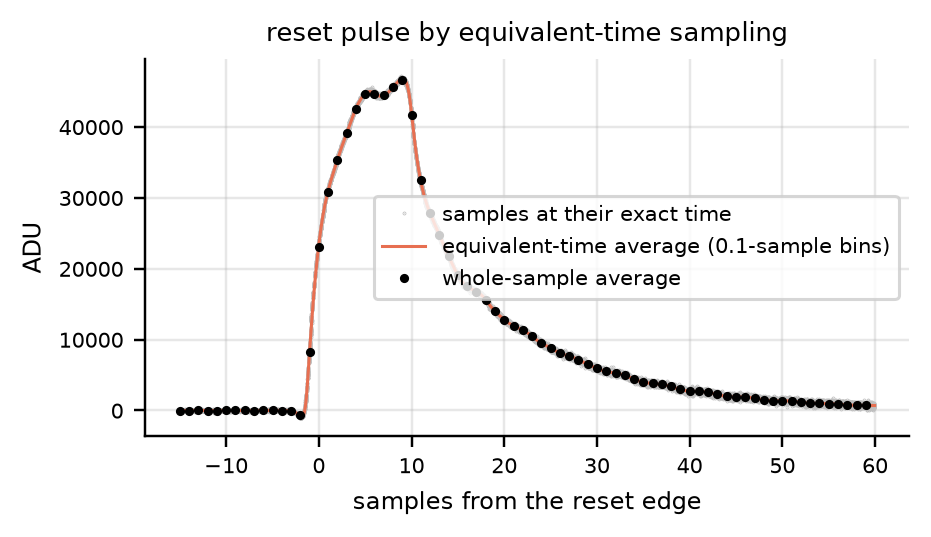
\includegraphics[width=0.62\textwidth]{edge_equivalent_time.png}
\caption{Equivalent-time pulse $E(\phi)$ (red) against whole-sample averages (dots).}
\end{figure}

\begin{figure}[H]
\centering
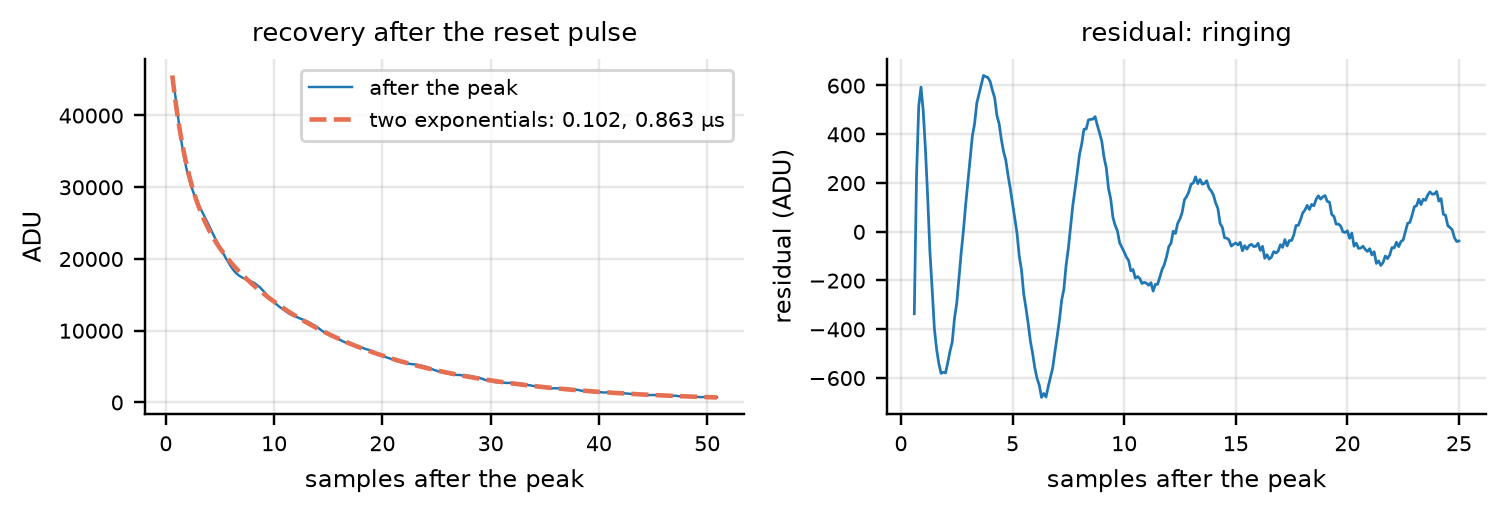
\includegraphics[width=\textwidth]{edge_recovery_ringing.png}
\caption{Two-exponential fit after the peak and its residual (the ringing).}
\end{figure}

\feat{edge: dip per volt SW (ADU/V)}{ADU/V}
Per pixel, with the template from $\ko$: dip $= \min_{\nw \le \tau < s} m_\tau$, divided by the summing-well swing
$\code{SW\_1\_H} - \code{SW\_1\_L}$ from the \code{.meta}. \code{edge: pulse per volt RG (ADU/V)}: pulse
$= \max_{\tau \ge e} m_\tau - \mean_{e - q' \le \tau < e} m_\tau$, $q' = \min(20, \max(1, \lfloor\nw/4\rfloor))$, divided by
$\code{RG\_1\_H} - \code{RG\_1\_L}$. \code{edge: pulse/dip ratio}: pulse/dip, in which the common amplification cancels.

\paragraph{Variation along the cycle.} $\Sigma_\tau = \mean_{p}\,\std_{k \ge \ko}\bigl(Y_{k,\tau} - b_k\bigr)$ (ddof 0), the
skip-to-skip scatter at each position.
\feat{edge: cycle variation in signal window (ADU)}{ADU}
$\med_{s \le \tau < e}\Sigma_\tau$. \code{at dip}: $\max_{\nw \le \tau < s}\Sigma_\tau$. \code{at reset}:
$\max \Sigma_\tau$ over $[\max(e, \tau_\text{pk} - 17), \min(P, \tau_\text{pk} + 23))$. \code{after reset}: $\med_{\tau \ge \tau_\text{pk} + 46}\Sigma_\tau$.
On steep edges $\Sigma_\tau \approx |\partial_\tau M| \times$ (timing jitter and the sub-sample walk), so it measures timing $\times$
slope; inside the windows it measures the noise that enters the CDS.

\begin{figure}[H]
\centering
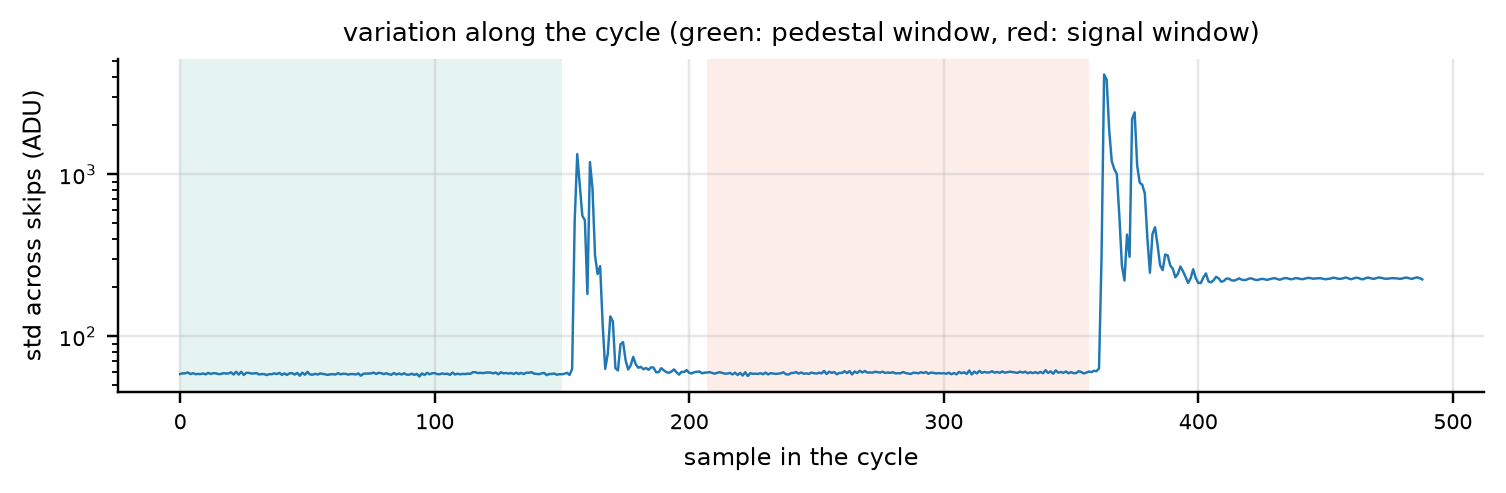
\includegraphics[width=\textwidth]{edge_cycle_variation.png}
\caption{$\Sigma_\tau$ with the pedestal (green) and signal (red) windows.}
\end{figure}

%======================================================================
\section{Slow structure (group \code{slow})}

\feat{slow: row-start recovery time (skips)}{skips}
Take the first row-start pixel $r > 0$ whose next pixel $r + 1$ is not a row start (else $r = 0$). Then
$d_k = b_{r,k} - b_{r+1,k}$, $k < N$, and the fit $d_k = A e^{-k/\tau} + C$ with $\tau \in [2, \max(2000, 4N)]$ gives $\tau$;
\code{amplitude} is $A$. It measures how the electronics recover from the vertical clocking.
\feat{slow: drift (ADU/ms)}{ADU/ms}
Slope of $b_{p,\lfloor N/2\rfloor}$ against the time $t^\text{ped}_{p,\lfloor N/2\rfloor}/f_s$ (ms) over $p \in \G$ (needs $\ge 2$ pixels).
\feat{slow: H-transfer peak-to-peak (ADU)}{ADU}
Per pixel and transfer $a_{p,m} = \max_\tau h_{m,\tau} - \min_\tau h_{m,\tau}$ (baseline from $\min(30, \max(1,\lfloor L/10\rfloor))$
samples). Feature $\mean_p\mean_m a_{p,m}$; \code{first-to-last change} $= \mean_p (a_{p,M_p} - a_{p,1})$.
\feat{slow: PC1 variance fraction}{fraction}
The residual cycles of all usable pixels, stacked ($\sum_p (N - \ko)$ rows $\times$ $P$ columns) and centred, have singular values
$s_1 \ge s_2 \ge \dots$; PC$i$ fraction $= s_i^2/\sum_j s_j^2$, $i = 1, 2, 3$. On real traces PC1 ($\sim$82\,\%) is the sub-sample phase
walk at the edges, and PC2 is the level shift set by each reset.

\begin{figure}[H]
\centering
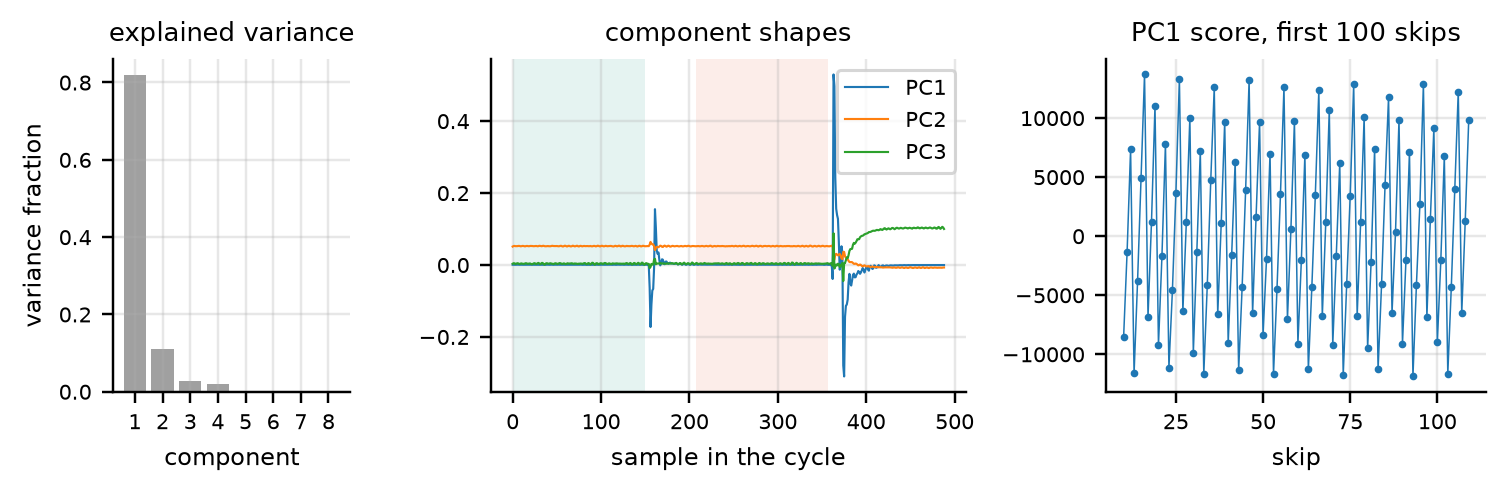
\includegraphics[width=\textwidth]{slow_principal_components.png}
\caption{Principal components of the residual cycles: explained variance, the first three components, the PC1 score of the first 100 skips.}
\end{figure}

%======================================================================
\section{The additions of 2026-10-21/22 (\code{trace\_features\_extra.py})}
\label{sec:extra}

The 56 scalar features and 4 curves added on 2026-10-21/22 are computed by \code{extra\_features(ctx)} in
\code{src/trace\_features\_extra.py}, called as block F at the end of \code{\_trace\_features}, after all other groups. They use the same
shared arrays as the other features (the \code{ctx} dictionary):

\begin{center}
\small
\begin{tabular}{>{\raggedright\arraybackslash}p{0.24\textwidth}>{\raggedright\arraybackslash}p{0.47\textwidth}l}
\toprule
\code{ctx} field & meaning & notation here \\
\midrule
\code{Cm} & CDS of every pixel, pixels $\times$ skips (equal lengths $N$) & $c_{p,k}$ \\
\code{cyc}, \code{res} & raw cycles of every pixel; residual cycles of the usable pixels (skips $\ge \ko$) & $Y_{k,\tau}$, $R_{k,\tau}$ \\
\code{det} & detrended CDS of the usable pixels (skips $\ge \ko$) & $r_{p,k}$, length $N' = N - \ko$ \\
\code{good}, \code{row\_starts} & usable and row-start pixels & $\G$, $\mathcal S$ \\
\code{n\_ped}, \code{sig}, \code{first}, \code{n} & window length, signal-window offset, first noise skip, skips & $\nw$, $s$, $\ko$, $N$ \\
\code{skip\_rate}, \code{sample\_rate} & $f_s/P_\text{exact}$, $f_s$ & $f_\text{skip}$, $f_s$ \\
\code{starts} & absolute first sample of every cycle & $t^\text{ped}_{p,k}$ \\
\code{common} & $\med_{p\in\G} c_{p,k}$ over all skips & $\hat c_k$ \\
\code{scalars}, \code{curves} & the features already computed (read only) & \\
\code{allan\_n} & the 13 block lengths $\{1,2,3,5,7,10,15,20,30,50,75,100,160\}$ & $n$ \\
\code{regions}, \code{trace} & the \code{TraceRegions} and the decoded trace (values and flags) & \\
\code{meta} & the \code{.meta} settings (may be empty) & \\
\bottomrule
\end{tabular}
\end{center}

\paragraph{Blocks and errors.} The additions are computed in seven blocks (\code{start}, \code{switching}, \code{shape}, \code{lines},
\code{levels}, \code{prepulse}, \code{clock}), each inside its own \code{try}. A block that raises an exception leaves its features
NaN and records the reason as \code{info["errors"]["extra: <block>"]}; the other blocks still run. Every scalar of the registry
exists in the result; one that was never set is NaN. Per-pixel values $f_p$ are reduced as in Section~2: $F = \med f_p$ (NaN values
ignored), spread $= \rsd f_p$.

\paragraph{Constants} (module level): \code{LATE} $= (20, 60)$, \code{FIRST\_SKIPS} $= 20$, \code{TRANSIENT\_SKIPS} $= 30$,
\code{MPENCIL\_ORDER} $= 4$. With them,
\begin{equation}
\mathcal K_L = \{k : \min(20, \lfloor N/5\rfloor) \le k < \min(60, N)\}\ [20\dots59],\qquad k_F = \min(20, N),\qquad
\tilde c_p = \med_{k \ge \ko} c_{p,k}.
\end{equation}

\subsection{Start of pixel (group \code{start}, block \code{start})}

\paragraph{In-window slope.} For every skip, the least-squares slope (ADU per sample) of the pedestal window and of the signal window
of the raw cycle, averaged:
\begin{equation}
\Delta_{p,k} = \tfrac12\bigl[\beta(Y_{k,0:\nw}) + \beta(Y_{k,s:s+\nw})\bigr],\qquad
\beta(y_{0:m}) = \frac{\sum_i (i - \bar\imath)(y_i - \bar y)}{\sum_i (i - \bar\imath)^2}.
\end{equation}
Write $\Delta^\text{late}_p = \med_{k \in \mathcal K_L}\Delta_{p,k}$, $x_{p,k} = \Delta_{p,k} - \Delta^\text{late}_p$ and
$y_{p,k} = c_{p,k} - \tilde c_p$.

\feat{start: CDS-slope lever arm (samples)}{samples}
Ordinary least squares $y_{p,k} = L\,x_{p,k} + a$ over $k < k_F$ and $p \in \G$, pooled. The feature is $L$. If the first-skip CDS
offset is pure baseline slope seen through the CDS, $L \approx -s$, minus the distance between the two window centres [$-207$].
\code{start: slope-explained fraction} $= 1 - \operatorname{var}(\text{residual})/\operatorname{var}(y)$ ($R^2$).
\feat{start: in-cycle slope at skip 0 (ADU/us)}{ADU/µs}
$x_{p,0}\cdot f_s/10^6$ per pixel; median.
\feat{start: transient time constant (us)}{µs}
Per pixel, $Y^b_{k,\tau} = Y_{k,\tau} - \tfrac{1}{\nw}\sum_{\tau'<\nw}Y_{k,\tau'}$ and
$d_\tau = Y^b_{0,\tau} - \mean_{k\in\mathcal K_L} Y^b_{k,\tau}$ (skip 0 minus the late mean waveform). One exponential
$d_\tau = A e^{-t/\tau_0} + C$ (Section~2.1) is fitted on the samples of the two windows,
$\tau \in [0, \nw) \cup [s, \min(s+\nw, P))$, with $t = \tau/f_s$ in µs and $\tau_0 \in [0.5, 200]$\,µs. Features: $\tau_0$ and
\code{start: transient amplitude (ADU)} $= A$ (the value at the start of the cycle); medians over $\G$.
\feat{start: first-skip excess per volt H (ADU/V)}{ADU/V}
\code{skip: first-skip CDS excess} divided by $\code{H1\_A\_H} - \code{H1\_A\_L}$ from the \code{.meta} (NaN without them or if equal).
The swing of \code{H1\_A} is used for every channel.
\feat{level: slope-corrected CDS rise (ADU)}{ADU}
With $\bar\Delta_k = \med_{p\in\G}\Delta_{p,k}$ and $K = \max(1,\lfloor N/10\rfloor)$:
\code{level: common CDS rise} $- L\,\bigl(\mean_{k \ge N-K}\bar\Delta_k - \mean_{\ko \le k < \ko+K}\bar\Delta_k\bigr)$ (needs $N - K \ge \ko + K$).
\feat{start: row-start/inner first-skip ratio}{---}
With $E_p = c_{p,0} - \tilde c_p$ for every pixel: $\med_{p\in\mathcal S} E_p \,/\, \med_{p\in\G} E_p$.
\feat{start: reset jump skip 0 to 1 (ADU)}{ADU}
$\tfrac{1}{\nw}\sum_{\tau<\nw}(Y_{1,\tau} - Y_{0,\tau})$ per pixel (raw pedestal means of skips 1 and 0); median.
\paragraph{Mean transient (curve \code{start: mean transient}).} $T_k = \mean_{p\in\G}\, y_{p,k}$, $k = 0 \dots 29$.
\feat{start: transient amplitude, matched filter (ADU)}{ADU}
$\dfrac{\sum_{k<30} y_{p,k}T_k}{\sum_{k<30}T_k^2}\,\max_k|T_k|$ per pixel; median. The projection on the trace's own template has about
30\,\% less noise than $E_p$ alone.
\feat{start: mode frequency (kHz)}{kHz}
\textbf{Matrix pencil} of $T_0 \dots T_{29}$ ($M = 30$, order $q = 4$): the Hankel matrix $\mathbf Y_{ij} = T_{i+j}$,
$i = 0 \dots M - L - 1$, $j = 0 \dots L$, $L = \lfloor M/2\rfloor$; its SVD $\mathbf Y = U\Sigma V^\top$; $V_q$ = the first $q$ right
singular vectors; the poles $z$ are the eigenvalues of $V_{q,1}^+ V_{q,2}$ ($V_{q,1}$, $V_{q,2}$: $V_q$ without its last and first row);
the amplitudes $c$ solve $T_k \approx \sum_i c_i z_i^k$ by least squares. Among the poles with $\Im z > 10^{-6}$ and $0 < |z| < 1$, the one
with the largest $|c|$ gives $\arg z\, f_\text{skip}/(2\pi)$ (kHz) and \code{start: mode damping (us)} $= -10^6/(f_\text{skip}\ln|z|)$.
\code{start: fast decay (us)} $= -10^6/(f_\text{skip}\ln z)$ for the real pole ($|\Im z| \le 10^{-6}$) with $0 < z < e^{-1/10}$ (decaying within
10 skips) and the largest $|c|$. NaN when no such pole exists (often, for the fast decay).
\feat{start: ringing frequency (kHz)}{kHz}
\code{fit: first-skip ringing frequency (cyc/skip)} $\times f_\text{skip}/10^3$.

\subsection{Telegraph switching and jumps (block \code{switching})}

\paragraph{Null CDS.} With $h = \lfloor\nw/2\rfloor$ [75], a CDS between the two halves of the pedestal window of the residual cycles, where
no charge moves:
\begin{equation}
z_{p,k} = \tfrac1h\sum_{\tau<h}R_{k,\tau} - \tfrac1h\sum_{\tau=h}^{2h-1}R_{k,\tau},\qquad k \ge \ko .
\end{equation}
\code{noise: null-CDS noise (ADU)} $= \std_k z_{p,k}$ (ddof 0); \code{discrete: null-CDS kurtosis} $= \mean\tilde z^4/(\mean \tilde z^2)^2 - 3$
(NaN with $\le 3$ values or zero variance); \code{noise: null-CDS autocorrelation at lag 1} $=$ the Pearson correlation of
$(z_{p,k})$ with $(z_{p,k+1})$. Medians over $\G$.

\paragraph{In-window steps.} All windows of a pixel: the rows $R_{k,0:\nw}$ and $R_{k,s:s+\nw}$, $k \ge \ko$ [$2\times490$]. Each row
is cut into $m = \lfloor\nw/10\rfloor$ [15] blocks of 10 samples with means $\mu_j$. The block-mean noise is
$\sigma_b = \sqrt{v/10}$, with $v$ the median of the within-block variances (ddof 1) over all blocks and windows. For every split
$j = 1 \dots m-1$,
\begin{equation}
t_j = \frac{|\bar\mu_{[j,m)} - \bar\mu_{[0,j)}|}{\sigma_b\sqrt{1/j + 1/(m-j)}},
\end{equation}
and a window's best step is the split with the largest $t_j$. \code{discrete: in-window step rate (\%)} $= 100\times$ the fraction of
windows with best $t > 6$; \code{discrete: in-window step amplitude (ADU)} $=$ the median $|\bar\mu_{[j,m)} - \bar\mu_{[0,j)}|$ of those
windows (NaN if none). Medians over $\G$. The amplitude is NaN on most pixels without switching (about 58\,\% of the 2026-10-12 traces).

\paragraph{Jump-robust variance} (Andersen, Dobrev \& Schaumburg 2012) of $r = r_p$, length $N'$:
\begin{equation}
\text{MedRV} = \frac{\pi}{6 - 4\sqrt3 + \pi}\,\frac{N'}{N'-2}\sum_{k=1}^{N'-2}\med\bigl(|r_{k-1}|, |r_k|, |r_{k+1}|\bigr)^2
\end{equation}
(NaN for $N' < 5$). \code{noise: jump-robust CDS sigma (ADU)} $= \sqrt{\text{MedRV}/N'}$; \code{discrete: jump share of CDS variance}
$= \max\bigl(0,\ 1 - \text{MedRV}/\sum_k r_k^2\bigr)$. For Gaussian white noise these are $\approx \std(r)$ and $\approx 0.02$.
\feat{discrete: jump count (Lee-Mykland, 1 \%)}{count}
Window $K_\text{LM} = 20$ (NaN for $N' < 60$). For $k = K_\text{LM} \dots N'-1$, the local bipower variance from the previous skips
$\hat\sigma_k^2 = \frac{1}{K_\text{LM}-2}\sum_{j=k-K_\text{LM}+1}^{k-2}|r_{j+1}||r_j|$, $L_k = |r_k|/\hat\sigma_k$, and $k$ counts if
$(L_k - C_n)/S_n > \beta^\ast$ with $n = N'$, $c = \sqrt{2/\pi}$,
$C_n = \frac{\sqrt{2\ln n}}{c} - \frac{\ln\pi + \ln\ln n}{2c\sqrt{2\ln n}}$, $S_n = \frac{1}{c\sqrt{2\ln n}}$ and
$\beta^\ast = -\ln(-\ln 0.99) = 4.60$ (Lee \& Mykland 2008; the factor $c$ matches the bipower estimate, which is
$\tfrac2\pi\sigma^2$; it was missing before 2026-10-22). \emph{Caveat:} with a local window of only 20 skips the estimate
$\hat\sigma_k$ is noisy, so pure Gaussian noise still gives about 0.26 counts per pixel (simulated) rather than a 1\,\% rate:
the count is a relative measure of jumps.
\feat{discrete: STA/LTA maximum}{---}
On $q_k = r_k^2$: $\max_k \bigl(\tfrac15\sum_{i=k}^{k+4} q_i\bigr)\big/\bigl(\tfrac1{50}\sum_{i=k-50}^{k-1}q_i\bigr)$ over
$k = 50 \dots N'-6$ (NaN for $N' < 56$).
\feat{discrete: crest factor}{---}
$\max_k|r_k|/\std(r)$ (ddof 0).
\feat{noise: volatility clustering (Ljung-Box of e\^{}2, 10 lags)}{---}
On $q_k = r_k^2 - \overline{r^2}$: $Q = N'(N'+2)\sum_{\ell=1}^{10}\hat\rho_\ell^2/(N' - \ell)$, $\hat\rho_\ell = \sum_k q_kq_{k+\ell}/\sum_k q_k^2$.
\feat{discrete: whitened CDS kurtosis}{---}
$X = \mathrm{rfft}(r - \bar r)$, $\Pi_j = |X_j|^2$; $\Pi$ is smoothed by a 9-point moving average with 9 mirrored values at each end;
$w = \mathrm{irfft}(X/\sqrt{\Pi^\text{smooth}})$; feature $=$ the excess kurtosis of $w$ (NaN for $N' < 32$).
\feat{discrete: max within-window spectral kurtosis}{---}
On the pedestal windows of the residual cycles ($R_{k,0:\nw}$, at least 10 rows): $X_{k,j} = |\mathrm{rfft}(R_{k,0:\nw}\,h)_j|^2$ with a
Hann window $h$; $\mathrm{SK}_j = \mean_k X_{k,j}^2/(\mean_k X_{k,j})^2 - 2$; feature $\max_{j\ge1}\mathrm{SK}_j$ (0 for Gaussian noise).

\paragraph{Within-cycle structure function (curve).} On the pedestal windows $R_{k,0:\nw}$: $m = \lfloor\nw/15\rfloor$ [10] block means
$B_{k,j}$ of 15 samples (1\,µs), and
$D(\ell) = \sqrt{\mean_{k,j}(B_{k,j+\ell} - B_{k,j})^2}$, $\ell = 1\dots9$ (NaN where $\ell \ge m$); the curve is $\mean_{p\in\G}D_p(\ell)$.
\feat{noise: structure-function excess at 9 blocks (ADU)}{ADU}
$\sqrt{\max(D(9)^2 - D(1)^2, 0)}$ of that curve.

\subsection{Noise shape (block \code{shape})}

\paragraph{Hadamard deviation.} On $u_p$, the CDS with only the common pattern removed (Section~2; \emph{not} detrended), with disjoint
$n$-block means $\bar u_j$ ($m = \lfloor N'/n\rfloor \ge 4$, else NaN):
$\sigma_H(n) = \sqrt{\tfrac16\mean_j(\bar u_{j+2} - 2\bar u_{j+1} + \bar u_j)^2}$. The second difference cancels a linear drift, so no
polynomial is needed and the long blocks are not biased low. Curve \code{noise: Hadamard deviation}: $\mean_p\sigma_H(n)$ at the 13 values
of $n$ (NaN at $n = 160$ for $N' = 490$). \code{noise: Hadamard deviation n=50 (ADU)}: $\sigma_H(50)$ per pixel, median.
\paragraph{Modified Allan deviation (curve).} On $r_p$: running means $a_i$ of length $n$, $d_i = a_{i+n} - a_i$,
$\delta_j = \tfrac1n\sum_{i=j}^{j+n-1} d_i$, $\operatorname{MDEV}(n) = \sqrt{\tfrac12\mean_j\delta_j^2}$ (NaN if $N' < 3n+1$);
$\mean_p$ at the 13 values of $n$.
\feat{noise: 1/f corner frequency (kHz)}{kHz}
On the curve \code{noise: CDS spectrum, log frequency} $\bar S_i$ (spectrum of the $u_p$ in 40 log bins with centres
$f_i = \sqrt{e_ie_{i+1}}$), the model $\ln S = \ln(W + A f^{-\gamma})$ is fitted to $\ln \bar S_i$ against $\ln f_i$ (non-linear least squares,
$\gamma \in [0.2, 3]$, start $W = \med$ of the upper half of $\bar S$, $A = W f_1$, $\gamma = 1$). The corner
$f_c = (A/W)^{1/\gamma}$ is clipped to $[f_1/2,\ 2f_{40}]$ (a corner outside the band means ``no $1/f$ in the band'' or ``$1/f$ everywhere'');
reported in kHz. \code{noise: 1/f exponent} $= \gamma$. NaN with fewer than 6 finite positive bins or if the fit fails.
\feat{noise: Lorentzian corner (kHz)}{kHz}
The same data, model $\ln(W + B/(1 + (f/f_L)^2))$ against $f$ (linear), $f_L \in [f_1/10, 10f_{40}]$, start $f_L = \med f_i$;
$f_L$ in kHz.
\feat{noise: lag-1 autocorrelation of 10-skip means}{---}
$\rho(1)$ of the disjoint 10-skip means of $r_p$ (needs $\ge 5$ blocks); median.
\feat{noise: DFA exponent}{---}
Profile $y_k = \sum_{i\le k}(r_i - \bar r)$; for each scale $\sigma \in \{4,6,8,12,16,24,32,48\}$ with $\ge 4$ segments, the rms $F(\sigma)$ of
$y$ about a straight line fitted in each non-overlapping segment; the slope of $\ln F$ against $\ln\sigma$ (needs $\ge 3$ scales). White
noise: 0.5.
\feat{noise: CDS spectral slope}{---}
$\Pi_j = |\mathrm{rfft}((r - \bar r)h)_j|^2$, $j \ge 1$ (Hann window $h$): slope of $\ln\Pi_j$ against $\ln j$.
\code{noise: CDS spectral centroid} $= \sum_j (j/J)\Pi_j/\sum_j\Pi_j$ with $J$ the number of bins (a fraction of the Nyquist frequency).
\feat{noise: sample entropy}{---}
$r$ standardized; templates of length $m = 2$ and $3$ (the first $N'-2$ of each); $B$, $A$ = the number of pairs $i<j$ within Chebyshev
distance $0.2$; feature $-\ln(A/B)$ (NaN for $N' < 20$ or $A$ or $B = 0$).
\feat{noise: permutation entropy (m=4)}{---}
The ordinal pattern of every 4 consecutive values (delay 1); $-\sum p\ln p/\ln 4!$ over the observed patterns (needs $N' \ge 240$).
\feat{noise: red-noise beta (50 skips)}{---}
$\std(\text{50-skip block means})/(\std(r)/\sqrt{50})$, both ddof 1, $\ge 3$ blocks. White noise: 1.

\paragraph{Noise budget.} The residual cycles of all usable pixels are stacked, $\mathbf R$ ($\sum_p N'$ rows $\times$ $P$ columns), and
centred by column. The CDS weight vector is $w_\tau = +1/\nw$ for $\tau < \nw$, $-1/\nw$ for $s \le \tau < s + \nw$, else 0, so
$\mathbf R w$ is the CDS of the residuals. With the SVD $\mathbf R = U\Sigma V^\top$ (singular values $\varsigma_i$ in decreasing order:
the waveform modes by waveform variance), mode $i$ carries $\kappa_i = \varsigma_i^2 (v_i^\top w)^2$ of the CDS variance,
$\sum_i\kappa_i = \|\mathbf Rw\|^2$.
\code{noise: CDS variance share of the 3 largest waveform modes} $= (\kappa_1+\kappa_2+\kappa_3)/\sum\kappa$;
\code{noise: waveform modes for 90 \% of the CDS variance} $=$ the smallest $i$ with $\sum_{j\le i}\kappa_j \ge 0.9\sum\kappa$. If the signal window would run past the cycle ($s + \nw > P$) the block raises an error (the weights would not balance), so the noise-budget features are NaN.

\subsection{Pickup lines (block \code{lines})}

\paragraph{Multitaper F test} (Thomson 1982) on each $r_p$, $p\in\G$, all cut to the shortest length $n$: $K = 5$ DPSS tapers $v_k$ with
$NW = 3$ (unit energy), $U_k = \sum_t v_k(t)$, $Y_k(f) = \mathrm{rfft}(v_k\,(r - \bar r))$,
\begin{equation}
\mu(f) = \frac{\sum_k U_kY_k(f)}{\sum_kU_k^2},\qquad
F(f) = \frac{(K-1)\,|\mu|^2\sum_kU_k^2}{\sum_k|Y_k(f) - \mu U_k|^2},
\end{equation}
compared with $F_\text{crit} = F^{-1}_{2,\,2K-2}(1 - 0.001)$. The bins with $f \le 3f_\text{skip}/n$ (the taper bandwidth) are left out.
\code{discrete: line count (F-test, p<0.001)}: the number of bins where $F > F_\text{crit}$ in at least half of the pixels.
\code{strongest line frequency (kHz)}: $f_0 = \argmax_f\med_pF_p(f)$. \code{strongest line amplitude (ADU)}: $\med_p 2|\mu_p(f_0)|$.
\code{line phase coherence, pixel clock}: $|\mean_p e^{\mathrm i\varphi_p}|$ with $\varphi_p = \arg\mu_p(f_0)$ (referred to each pixel's
skip $\ko$); \code{absolute time}: $|\mean_p e^{\mathrm i(\varphi_p - 2\pi f_0t_p)}|$ with $t_p = t^\text{ped}_{p,\ko}/f_s$.
\feat{discrete: line frequency, whole trace (kHz)}{kHz}
Lomb--Scargle periodogram of all $r_{p,k}$ ($p\in\G$) at their absolute times $t^\text{ped}_{p,\ko+k}/f_s$, mean removed, on the grid
$200, 205, \dots$\,Hz up to $\min(15\,\text{kHz}, f_\text{skip}/2)$; the frequency of the maximum.

\subsection{Levels (block \code{levels})}

\feat{level: common-pattern amplitude spread}{---}
With $\gamma_k = \hat c_k - \mean_{k'\ge\ko}\hat c_{k'}$ ($k \ge \ko$): $a_p = \sum_k(c_{p,k} - \bar c_p)\gamma_k/\sum_k\gamma_k^2$;
feature $\rsd_{p\in\G}\,a_p$.
\feat{noise: baseline-CDS residual correlation}{---}
Pearson correlation of $\Dt(b_{p,\ko:N})$ (the per-skip pedestal means of the raw cycles, detrended) with $r_p$; median.

\subsection{The dip before the per-cycle pulse (block \code{prepulse}, group \code{edge})}

On the equivalent-time pulse $E(\phi)$ (Section~\ref{sec:edges}; 0.1-sample bins with centres $\phi_i = -15 + 0.05 + 0.1i$ samples,
$\phi = 0$ at the half-height crossing of the edge):
\begin{equation}
E_0 = \mean\{E(\phi_i) : -15 < \phi_i < -8\},\qquad
\text{depth} = \min\{E(\phi_i) : -6 < \phi_i < 0\} - E_0 .
\end{equation}
\begin{itemize}
\item \code{edge: pre-pulse dip depth (ADU)} $=$ depth (negative);
\item \code{edge: pre-pulse dip / pulse height} $=$ depth$/(\max_iE(\phi_i) - E_0)$, only if the pulse height is positive.
\end{itemize} On the 2026-10-12 traces the dip sits 120--130\,ns ($\approx$1.9 samples) before the crossing and is
about 1.5 samples wide, which is why single cycles show it as one low sample.

\subsection{Clocking regions (block \code{clock}, group \code{clock})}

\paragraph{The vertical block $V$} is \code{regions.v} (Section~1.1): the transfers of the vertical block before the first row-start pixel
after pixel 0 (the block before row 2), first transfer dropped when there are at least three, each transfer
$V_{m,\tau} = v_{t^V_m + \tau}$, $\tau < \mathrm{round}(P_V)$ with $P_V$ the median spacing of the vertical edges, and only transfers
that end before the block's first horizontal edge. If no pixel after pixel 0 starts a row (a one-row trace), \code{regions.v} falls back to
the leading block; the \code{clock:} V features are then NaN (since 2026-10-22), because the leading block is not repeatable. The horizontal stacks $H^{(p)}_{m,\tau}$ are \code{regions.h} (length $\mathrm{round}(P_H)$).

Write $\ell_m = \med_\tau V_{m,\tau}$ (the level of transfer $m$) and $a(T_m) = \max_\tau T_{m,\tau} - \min_\tau T_{m,\tau}$ (peak-to-peak
of one transfer, no baseline removed). Let $\mathcal I = \{p \notin \mathcal S : M_p \ge 5\}$ (pixels that do not start a row, with at
least 1 horizontal transfer; charged pixels are not excluded).
\feat{clock: V-block level slope (ADU/transfer)}{ADU/transfer}
Least-squares slope of $\ell_m$ against $m$ (needs $\ge 3$ transfers in $V$, i.e.\ NPBIN $\ge 4$; NaN at 1$\times$1).
\feat{clock: V-transfer peak-to-peak (ADU)}{ADU}
$a_V = \med_m a(V_m)$ (needs $\ge 1$ transfer: at 1$\times$1 binning the single V transfer before row 2).
\feat{clock: H/V peak-to-peak ratio}{---}
$\med\{a(H^{(p)}_m) : p\in\mathcal I,\ \text{all } m\}/a_V$.
\feat{clock: first H block of a row, excess (ADU)}{ADU}
For every row-start pixel $p > 0$ whose H block has $M_p \ge 10$ transfers (the prescan burst,
$\code{NSBIN}\,(\code{NCOLPRE}+1)$ transfers), $\tfrac15\sum_{m<5} a(H^{(p)}_m) - \med_{m \ge \lfloor M_p/2\rfloor} a(H^{(p)}_m)$: the
first five transfers after coming off the row against the settled second half of the same block; the mean over those pixels.
(Since 2026-10-23, so that it works at 1$\times$1 binning; before, the first five transfers were compared with the other pixels'
blocks, which needs $\ge 5$ H transfers per pixel.)
\feat{clock: leading V-block level slope (ADU/transfer)}{ADU/transfer}
The block the trace starts in: the rising edges of flag bit 7 (bit 5 if bit 7 has fewer than two), lasting $\ge 10$ samples, before the
first rising edge of bit 6 in the trace (else before the first pedestal window). Transfers $v_{t:t+\mathrm{round}(P_V)}$ that end before that
point; if there are at least 13, the slope of $\ell_m$ over the last 12. Stored only (tier 2): the trace starts at a random point inside
this block (14--19 of its 20 transfers recorded on 2026-10-12), so the slope depends on what preceded the acquisition.

%======================================================================
\section{The curves}

\begin{longtable}{>{\raggedright\arraybackslash}p{0.3\textwidth}>{\raggedright\arraybackslash}p{0.63\textwidth}}
\toprule
Curve & Definition \\
\midrule
\endhead
\code{skip: mean shape} & $\med_{p \in \G} m^{(p)}_\tau$, block-averaged to $\le 500$ points \\
\code{skip: baseline droop curve} & $\med_p (b_{p,k} - b_{p,1})$, $k = 1 \dots N - 1$ \\
\code{horizontal: mean shape} & $\med_p \bar h^{(p)}_\tau$ \\
\code{vertical: mean shape} & $\med$ over transfers of $h_{m,\tau}$ \\
\code{level: common CDS pattern} & $\hat c_k$, $k = 0 \dots N-1$ \\
\code{noise: CDS autocorrelation} & $\mean_p \rho_p(\ell)$, $\ell = 1 \dots 50$ \\
\code{noise: Allan deviation} & $\mean_p \sigma_A(n)$ at the 13 values of $n$ \\
\code{noise: CDS spectrum} & $S(f)$ of the $r_p$, $0 \le f \le f_N$ \\
\code{noise: Allan deviation, common pattern removed} & $\mean_p \sigma^\text{ov}_A(n)$ of the $u_p$, at the 13 values of $n$ \\
\code{noise: CDS spectrum, log frequency} & $S(f)$ of the $u_p$, averaged in 40 bins with edges $e_j = f_1 (f_N/f_1)^{j/40}$ (empty bins
  interpolated in $\log f$) \\
\code{noise: within-cycle spectrum} & $S_\text{in}(f)$, $0 \le f \le 7.5$\,MHz \\
\code{noise: noise vs window length} & $\mean_p \sigma(L, 0)$, $L \in \mathcal L$ \\
\code{edge: equivalent-time pulse} & $E(\phi)$, $-15 \le \phi < 60$ in 0.1-sample bins \\
\code{edge: variation along the cycle} & $\Sigma_\tau$, $\tau = 0 \dots P-1$ \\
\midrule
\multicolumn{2}{l}{\emph{added 2026-10-21 (Section~\ref{sec:extra})}} \\
\code{start: mean transient} & $T_k = \mean_{p\in\G}(c_{p,k} - \tilde c_p)$, $k = 0 \dots 29$ \\
\code{noise: Hadamard deviation} & $\mean_p\sigma_H(n)$ of the $u_p$, at the 13 values of $n$ \\
\code{noise: within-cycle structure function} & $\mean_p D_p(\ell)$, $\ell = 1\dots9$ blocks of 15 samples \\
\code{noise: modified Allan deviation} & $\mean_p\operatorname{MDEV}(n)$ of the $r_p$, at the 13 values of $n$ \\
\bottomrule
\end{longtable}

\begin{figure}[H]
\centering
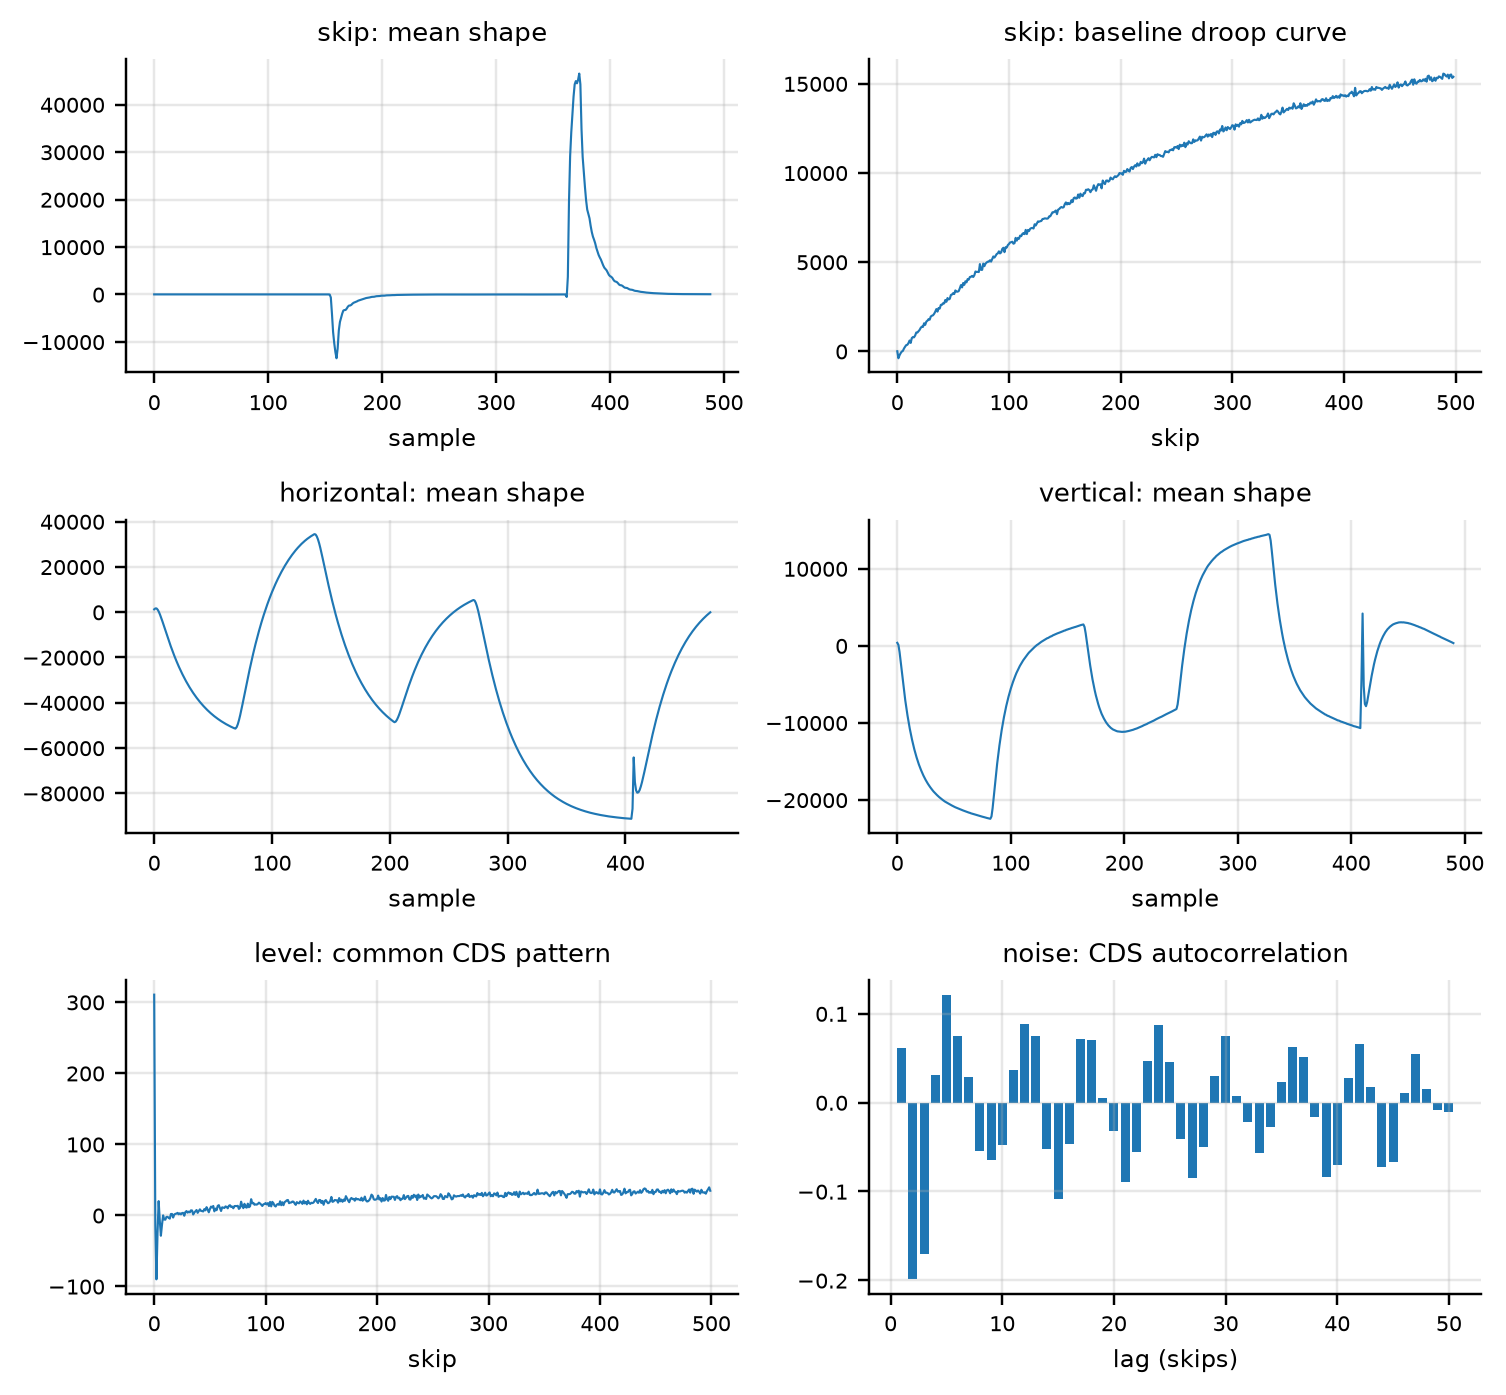
\includegraphics[width=\textwidth,height=0.8\textheight,keepaspectratio]{all_curves_a.png}
\caption{Curves 1--7 of the example trace (the 14 original curves; the 4 added ones are shown in the 2026-10-21 write-up).}
\end{figure}
\begin{figure}[H]
\centering
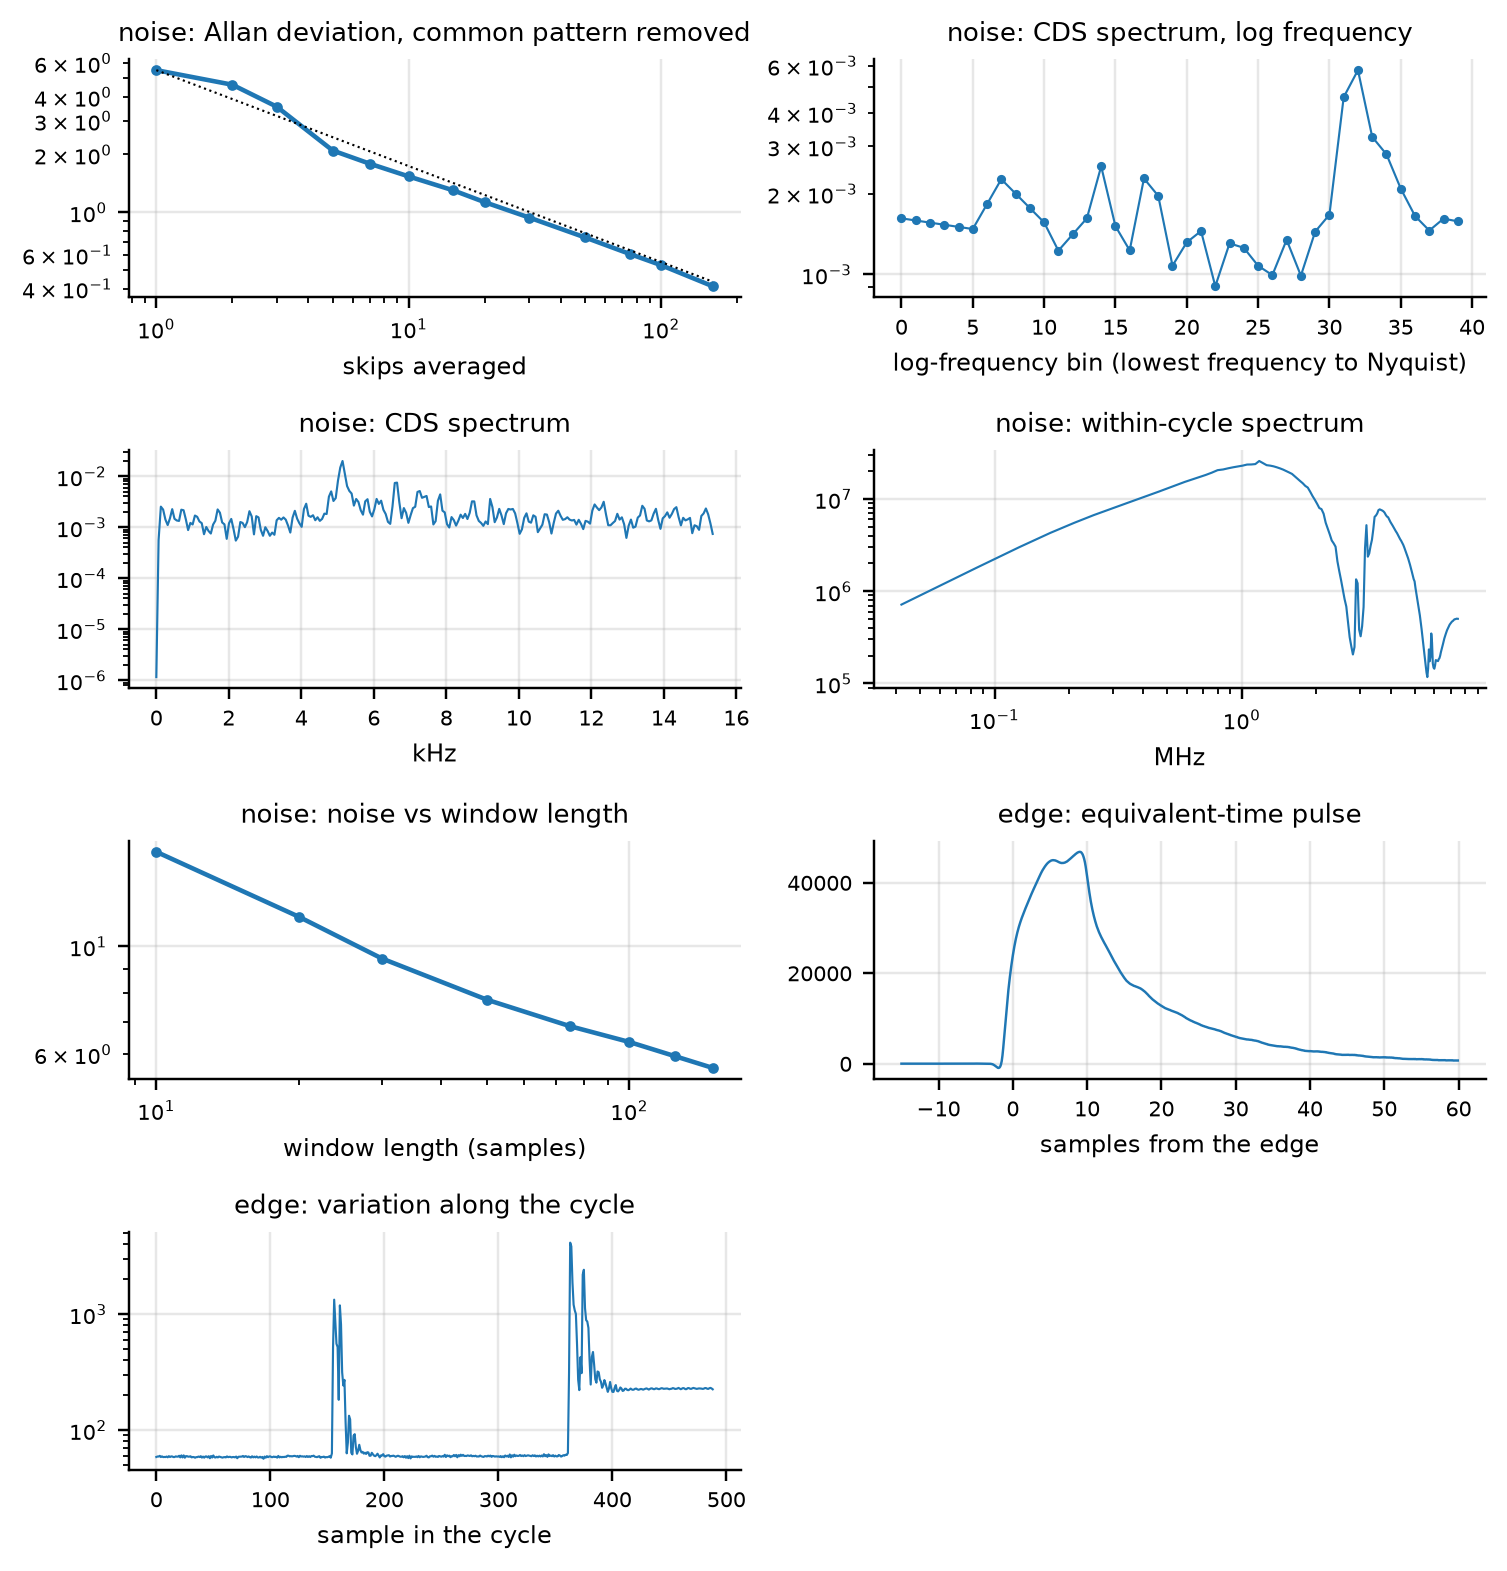
\includegraphics[width=\textwidth,height=0.8\textheight,keepaspectratio]{all_curves_b.png}
\caption{Curves 8--14 of the example trace (the dotted lines are white noise).}
\end{figure}

%======================================================================
\section{From one trace to a packet's features}

A packet has $n$ repeated trace sets at $\theta$ [10] and $n_\text{ref}$ at the reference [5], one trace per channel each.
The function \code{combine\_repeats} of \code{process\_packet.py} combines, per channel and feature, the values $f_1 \dots f_n$ of the usable traces:
\begin{itemize}
\item if $n \ge 5$, values with $|f_i - \med f| > 5\,\rsd(f)$ are left out (and counted in \code{n\_rejected});
\item \code{trace.}$f = \bar f$ over the kept values, \code{trace\_sd.}$f = \std(f)$ (ddof 1);
\item the same for the reference: \code{ref.}$f$, \code{ref\_sd.}$f$;
\item \code{diff.}$f = $ \code{trace.}$f - $ \code{ref.}$f$.
\end{itemize}
The scatter \code{trace\_sd} is the feature's measurement noise, used to judge changes (separation $=|\Delta\bar f|/s_\text{pooled}$) and
to weight features in the models.

%======================================================================
\section{Implementation tiers and evidence tiers}
\label{sec:tiers}

\paragraph{Implementation tier.} Every registry entry \code{FEATURES[name]} is a \code{Feature(group, unit, description, link, kind,
origin, tier)}. \code{origin} is \code{"comparison"} (\code{compare\_trace.py}), \code{"advanced"} (\code{trace\_features.py}) or
\code{"extra"} (\code{trace\_features\_extra.py}). \code{tier} is 0 for the original features, 1 for the implement-first additions and 2 for
the candidate additions; \code{names\_by\_tier(tiers=(0,1,2), kind="scalar")} lists the names of the given tiers and kind in registry order.

\begin{center}
\small
\begin{tabular}{lc>{\raggedright\arraybackslash}p{0.55\textwidth}}
\toprule
implementation tier & scalars & curves \\
\midrule
0 (original) & 85 & 14 \\
1 (2026-10-21/22) & 29 & 2 (\code{start: mean transient}, \code{noise: Hadamard deviation}) \\
2 (2026-10-21/22) & 27 & 2 (\code{noise: within-cycle structure function}, \code{noise: modified Allan deviation}) \\
\midrule
total & 141 & 18 \\
\bottomrule
\end{tabular}
\end{center}
By group, the 56 new scalars are: \code{noise} 19, \code{discrete} 15, \code{start} 13, \code{clock} 5, \code{level} 2, \code{edge} 2.

\paragraph{Evidence tiers.} They are computed by \code{lvl1/feature\_study.py} and need no labels.

\noindent Output: \code{lvl1/feature\_study/evidence\_tiers.json} and \code{feature\_table.csv}.

\noindent Data: the 59 usable traces of board 101 from the packet tests of 2026-10-12 (5 settings $\times$ 3 repeats $\times$ 4
amplifiers, one damaged ch3 trace left out), in \code{docs/slides/data/oct12\_trace\_features.csv}.

\noindent For each scalar $x$:
\begin{itemize}
\item \textbf{One-way ANOVA} $F = \dfrac{\sum_g n_g(\bar x_g - \bar x)^2/(G-1)}{\sum_g\sum_{i\in g}(x_i - \bar x_g)^2/(n - G)}$ over the
  groups with at least 2 finite values (NaN with fewer than 2 groups; $\infty$ if the within term is 0 and the between term is not).
\item \textbf{Settings $F$}: over the 4 \emph{changed} settings (VDD $-20.5$\,V, V low rails + TG, all H low rails, H3\_A\_L only; all
  taken with \code{NCOLPRE} 185, so the reference's \code{NCOLPRE} 0 cannot fake a separation), separately for ch0, ch1 and ch3; the minimum
  and the median of the three. With df $(3, 8)$, $F > 4$ means $p < 0.05$.
\item \textbf{Amplifier $F$}: over the 4 amplifiers within each of the 5 settings; the median of the five.
\item \textbf{Repeat share} $=\dfrac{\sum_{(g,\text{ch})}(n_{g,\text{ch}} - 1)s^2_{g,\text{ch}}/\sum(n_{g,\text{ch}} - 1)}{s^2_\text{all}}$ (ddof 1
  throughout): 0 = perfectly repeatable, about 1 = pure repeat scatter.
\item \textbf{NaN share} and \textbf{constant} (zero spread).
\item \textbf{Redundancy clusters}: over the features with $> 80$\,\% finite values and non-zero spread, $|\rho|$ = the absolute Spearman
  correlation across the 59 traces (Pearson correlation of the ranks; NaN set to 0); distance $1 - |\rho|$; average-linkage hierarchical
  clustering cut at distance 0.05 (on average $|\rho| > 0.95$).
\item \textbf{Informativeness} $= \ln(1 + \max(F_\text{set,min}, 0)) + \ln(1 + \max(F_\text{amp}, 0))$ (NaN counted as 0). The
  \textbf{representative} of a cluster is its most informative member; a feature outside the clustering counts as a representative.
\end{itemize}
The rules, applied in this order:
\begin{center}
\small
\begin{tabular}{lp{0.7\textwidth}}
\toprule
tier & rule \\
\midrule
C & constant, or NaN share $> 0.2$, or neither $F_\text{set,min} > 4$ nor $F_\text{amp} > 4$ \\
A & $F_\text{set,min} > 10$ or $F_\text{amp} > 10$, and repeat share $< 0.5$, and the representative of its cluster \\
B & all others (informative but redundant, or only $F$ 4--10, or repeat share $\ge 0.5$ or NaN) \\
\bottomrule
\end{tabular}
\end{center}
A is then sorted by informativeness and split into \textbf{A1} (the first $\lceil|A|/2\rceil$) and \textbf{A2} (the rest), so that the four
tiers have similar sizes. \textbf{P (protected)} is a fixed list (\code{PROTECTED}), chosen by physics, not by these data, and written
besides the evidence tiers:
\begin{itemize}[before=\raggedright]
\item $\sigma_e$: \code{skip: CDS rms (detrended)}, \code{fit: white noise per skip (ADU)}, \code{noise: jump-robust CDS sigma (ADU)},
  \code{noise: null-CDS noise (ADU)}, \code{noise: Allan deviation n=50 (ADU)};
\item gain: \code{noise: reset-level scatter (ADU)}, \code{edge: pulse per volt RG (ADU/V)}, \code{edge: dip per volt SW (ADU/V)}.
\end{itemize}
It exists because the evidence tiers reward
separating the traces, not predicting the labels, and on these 59 traces the amplifier dominates every correlation: without it the most
direct $\sigma_e$ estimator (CDS rms) and the kTC noise (reset-level scatter) are in B.

\begin{center}
\small
\begin{tabular}{lccccc}
\toprule
implementation tier & A1 & A2 & B & C & total \\
\midrule
0 & 27 & 19 & 22 & 17 & 85 \\
1 & 8 & 8 & 4 & 9 & 29 \\
2 & 2 & 9 & 7 & 9 & 27 \\
\midrule
total & 37 & 36 & 33 & 35 & 141 \\
\bottomrule
\end{tabular}
\end{center}
\code{lvl1/train\_lvl1.py} reads these labels (A = A1 + A2, and \code{impl0/1/2} from the implementation tier) to choose the trace features
each model sees (\code{--feature-tiers}, \code{--tier-ablation}, \code{--feature-ladder}); the per-model defaults are \code{MODEL\_TIERS} there.

%======================================================================
\section{Summary of the conventions}
\begin{itemize}
\item Medians over pixels or transfers, and $\rsd$ for spreads, keep single bad pixels from dominating.
\item Noise features use $r$ (polynomial-detrended CDS from skip $\ko$), never a running mean.
\item Times: samples $\times 1/15$ = µs, $\times 10^9/f_s$ = ns. Frequencies are scaled to the skip rate where they depend on it.
\item Every count follows the trace's own geometry (Section~1.2); impossible features are NaN, not zero.
\item Fits are least squares in the linear parameters with a grid-and-parabola search in the nonlinear ones, so they never get stuck
  at a grid point (the $1/f$ and Lorentzian fits of Section~\ref{sec:extra} use bounded non-linear least squares instead).
\item Groups, and the blocks of the 2026-10-21 additions, fail independently: a failure leaves that group's features NaN and is recorded in
  \code{info["errors"]}; the rest of the trace is still computed.
\item Every feature has an implementation tier (0, 1, 2); the evidence tiers (A1, A2, B, C) and the protected set P are computed from
  real traces without labels (Section~\ref{sec:tiers}).
\end{itemize}

\end{document}
